\documentclass[a4paper]{article}

\def\nbook {Applied Partial Differential Equations \\ with Fourier Series and Boundary Value Problems}
\def\nbookshort {APDeq}

\input{../headerapde}
\hfuzz=125pt  % ignore overfull boxes up to 5pt
\hbadness=10000 % suppress underfull warnings

\usetikzlibrary{arrows.meta, calc, decorations.markings, backgrounds}
\usepackage{esint}

\begin{document}
\maketitle

\newpage
\tableofcontents

\newpage
\section{\textsf{1 - Heat Equation}}

\subsection{\textsf{1.2 - Derivation of the Conduction of Heat in a One-Dimensional Rod}}
% QUESTION 1
\qs{1.2.1}{Briefly explain the minus sign:
\begin{enumerate}[label=(\alph*)]
	\item in conservation law (1.2.3) or (1.2.5) if \( Q = 0 \)
	\item in Fourier's law (1.2.8)
	\item in conservation law (1.2.12), \( \frac{\partial u}{\partial t} = -\frac{\partial \phi}{\partial x} \)
	\item in Fick's law (1.2.13)
\end{enumerate}}

\begin{enumerate}[label=(\alph*)]
	\item Assuming zero internal thermal energy, we have
	\[
		\frac{\partial e}{\partial t} = -\frac{\partial \phi}{\partial x} 
	\]
	The temporal change in thermal energy density is opposite to the spatial change in heat flux. If more heat leaves a unit volume than had entered, the thermal energy density decreases, and vice-versa.
	\item Fourier's law of heat conduction states
	\[
		\phi = -K_{0}\frac{\partial u}{\partial x} 
	\]
	Heat moves in the direction of the negative of the temperature gradient, or from hot to cold regions.
	\item The spatial change in heat flux is opposite to the temporal change in temperature. If more heat leaves a unit volume than had entered, the temperature decreases, and vice-versa.
	\item Fick's law states
	\[
		\phi = -k \frac{\partial u}{\partial x} 
	\]
	The chemical moves in the direction of the negative of the gradient of the chemical concentration, or from more to less concentrated regions.
\end{enumerate}

% QUESTION 2
\qs{1.2.2}{Derive the heat equation for a rod assuming constant thermal properties and no sources.
\begin{enumerate}[label=(\alph*)]
	\item Consider the total thermal energy between \( x \) and \( x + \Delta x \).
	\item Consider the total thermal energy between \( x = a \) and \( x = b \).
\end{enumerate}}

\begin{enumerate}[label=(\alph*)]
	\item For a thin slice of width \( \Delta x \), the rate of change of heat energy is approximately equal to the flow of thermal energy at \( x \) and \( x + \Delta x \).
	\[
		\frac{\partial }{\partial t} \!\left[ e \!\left( x,t \right)A \Delta x \right] \approx \phi \!\left( x, t \right)A - \phi \!\left( x + \Delta x, t \right)A
	\]
	Divide through by \( A \Delta x \) and in the limit as \( \Delta x \rightarrow 0 \), we find
	\[
		\frac{\partial e}{\partial t} = \lim\limits_{\Delta x \to 0} \frac{\phi \!\left( x, t \right) - \phi \!\left( x + \Delta x, t \right)}{\Delta x} = -\frac{\partial \phi}{\partial x}
	\]
	Replacing \( \partial e / \partial t \) with \( c \rho \partial u / \partial t \), where \( c \) is the specific heat and \( \rho \) is the mass density, we have
	\[
		c \rho \frac{\partial u}{\partial t} = -\frac{\partial \phi}{\partial x} 
	\]
	Lastly, we take the spatial derivative of Fourier's law, where \( K_{0} \) is the thermal conductivity
	\[
		\phi = -K_{0}\frac{\partial u}{\partial x} \quad \implies \quad \frac{\partial \phi}{\partial x} = -K_{0}\frac{\partial^{2}u}{\partial x^{2}} 
	\]
	and substitute into the conservation equation to derive the heat equation.
	\[
		\frac{\partial u}{\partial t} = \frac{K_{0}}{c \rho}\frac{\partial^{2}u}{\partial x^{2}} 
	\]
	\item In lieu of the approximation in the previous set-up, consider the integral conservation
	\[
		\frac{d }{d t}\int^{b}_{a} e \!\left( x,t \right) \, dx = \phi \!\left( a,t \right) - \phi \!\left( b,t \right)
	\]
	By the Fundamental Theorem of Calculus and the constancy of \( x \), the left side becomes
	\[
		\int^{b}_{a} \frac{\partial e}{\partial t} \, dx  
	\]
	And the right side
	\[
		-\int^{b}_{a} \frac{\partial \phi}{\partial x} \, dx  
	\]
	Setting equal and combining terms, we find
	\[
		\int^{b}_{a} \!\left[ \frac{\partial e}{\partial t} + \frac{\partial \phi}{\partial x} \right] \, dx = 0
	\]
	from which we can immediately deduce the conservation law. Proceed as in part (a).
\end{enumerate}

\newpage
% QUESTION 3
\qs{1.2.3}{Derive the heat equation for a rod assuming constant thermal properties with variable cross-sectional area \( A \!\left( x \right) \) assuming no sources by considering the total thermal energy between \( x = a \) and \( x = b \).}

By the integral conservation law, we have
\[
	\frac{d }{d t} \int^{b}_{a} e A \!\left( x \right) \, dx = \int^{b}_{a} \frac{\partial e}{\partial t}A \!\left( x \right) \, dx = -\int^{b}_{a} \frac{\partial }{\partial x}\!\left[ \phi \!\left( x,t \right)A \!\left( x \right) \right] \, dx   
\]
From which we can derive
\[
	\frac{\partial e}{\partial t}A \!\left( x \right) + \frac{\partial }{\partial x}\!\left[ \phi \!\left( x,t \right)A \!\left( x \right) \right] = 0 
\]
Replacing \( e \!\left( x,t \right) \) with \( c \rho u \!\left( x,t \right) \) and combining with the Fourier law, conclude
\[
	\frac{\partial u}{\partial t} = \frac{K_{0}}{c \rho A \!\left( x \right)}\frac{\partial }{\partial x}\!\left[ A \!\left( x \right)\frac{\partial u}{\partial x} \right] = \frac{K_{0}}{c \rho} \!\left[ \frac{\partial^{2}u}{\partial x^{2}} + \frac{1}{A \!\left( x \right)}\frac{\partial u}{\partial x}\frac{\partial A}{\partial x} \right]
\]

% QUESTION 4
\qs{1.2.4}{Derive the diffusion equation for a chemical pollutant.
\begin{enumerate}[label=(\alph*)]
	\item Consider the total amount of the chemical in a thin region between \( x \) and \( x + \Delta x \).
	\item Consider the total amount of the chemical between \( x = a \) and \( x = b \).
\end{enumerate}}

\begin{enumerate}[label=(\alph*)]
	\item The derivation is analogous to that of the heat equation for a thin slice, with chemical diffusivity \( k \) in lieu of the thermal diffusivity \( K_{0} / c \rho \).
	\item See 1.2.2(b) with the same comment about the chemical diffusivity as above.
\end{enumerate}

% QUESTION 5
\qs{1.2.5}{Derive an equation for the concentration \( u \!\left( x,t \right) \) of a chemical pollutant if the chemical is produced due to chemical reaction at the rate of \( \alpha u \!\left( \beta - u \right) \) per unit volume.}

One conceptual understanding here is the production of the chemical originates from some \textit{source} \( Q \), which from the conservation law gives us
\[
	\frac{\partial u}{\partial t} + \frac{\partial \phi}{\partial x} = \alpha u \!\left( \beta - u \right)
\]
From Fick's law, substitute \( \phi \) to derive
\[
	\frac{\partial u}{\partial t} - k \frac{\partial^{2}u}{\partial x^{2}} = \alpha u \!\left( \beta - u \right) 
\]
Observe the logistic form on the right. This equation is called the \textbf{Fisher-KPP equation}, named after Ronald Fisher, Andrey Kolmogorov, Ivan Petrovsky, and Nikolai Piskunov.

% QUESTION 6
\qs{1.2.6}{Suppose that the specific heat is a function of position and temperature, \( c \!\left( x,u \right) \).
\begin{enumerate}[label=(\alph*)]
	\item Show that the heat energy per unit mass necessary to raise the temperature of a thin slice of thickness \( \Delta x \) from \( 0^{\circ} \) to \( u \!\left( x,t \right) \) is not \( c \!\left( x \right)u \!\left( x,t \right) \), but instead \( \int^{u}_{0} c \!\left( x,\overline{u} \right) \, d \overline{u} \).
	\item Rederive the heat equation in this case. Show that (1.2.3) remains unchanged.
\end{enumerate}}

\begin{enumerate}[label=(\alph*)]
	\item Since specific heat is, in this instance, a function of temperature and not independent of it, we must integrate with respect to a dummy variable \( \overline{u} \):
	\[
		\int^{u}_{0} c \!\left( x,\overline{u} \right) \, d \overline{u}  
	\]
	Conceptually, the specific heat varies as a function of the temperature for any given \( \!\left( x,t \right) \). For infinitesimal subdivisions of the total change in temperature from \( 0 \) to \( u \), some amount of energy per unit mass \( c \!\left( x,\overline{u} \right) \, d \overline{u} \) is needed. Because this energy per unit mass varies depending on how far we are along the temperature change to \( u \), we integrate to sum those infinitesimal amounts.
	\item The beginning of the derivation proceeds as in the original case: conservation of heat energy mandates that the rate of change of heat energy equals the thermal flux through the boundaries and internal sources.
	\[
		\frac{\partial }{\partial t} \!\left[ e \!\left( x,t \right)A \Delta x \right] \approx \phi \!\left( x,t \right)A - \phi \!\left( x + \Delta x,t \right)A + Q \!\left( x,t \right)A \Delta x
	\]
	which implies equation (1.2.3)
	\[
		\frac{\partial e}{\partial t} + \frac{\partial \phi}{\partial x} = Q 
	\]
	However, what changes is in the calculation of thermal energy density. Instead of the product of specific heat, mass density, and temperature, we have
	\[
		e \!\left( x,t \right) = \rho \!\left( x \right) \int^{u}_{0} c \!\left( x,\overline{u} \right) \, d \overline{u} 
	\]
	Taking the time derivative and applying Leibniz's rule, derive
	\begin{align*}
		\frac{\partial e}{\partial t} & = \rho \!\left( x \right) \frac{\partial }{\partial t}\int^{u}_{0} c \!\left( x,\overline{u} \right) \, d \overline{u} \\
					      & = \rho \!\left( x \right)\!\left[ c \!\left( x,u \right) \frac{\partial u}{\partial t} + \!\left( x \right)\int^{u}_{0} \underbrace{\frac{\partial }{\partial t}c \!\left( x,\overline{u} \right)}_{= 0} \, d \overline{u} \right]
	\end{align*}
	which is analogous to our derivation of the heat equation in the original case. Combine with Fourier's law to get
	\[
		c \!\left( x,u \right) \rho \!\left( x \right) \frac{\partial u}{\partial t} = \frac{\partial }{\partial x} \!\left( K_{0} \frac{\partial u}{\partial x} \right) + Q
	\]
\end{enumerate}

% QUESTION 7
\qs{1.2.7}{Consider conservation of thermal energy (1.2.4) for any segment of a one-dimensional rod \( a \le x \le b \). By using the fundamental theorem of calculus,
\[
	\frac{\partial }{\partial b} \int^{b}_{a} f \!\left( x \right) \, dx = f \!\left( b \right) 
\]
derive the heat equation (1.2.9).}

The formula implies that \( a \) is constant and \( b \) is varying. Take our integral conservation law, and differentiate both sides by \( b \):
\begin{align*}
	\frac{\partial }{\partial b} \int^{b}_{a} \frac{\partial e \!\left( x,t \right)}{\partial t} \, dx & = \frac{\partial }{\partial b} \!\left[ \phi \!\left( a,t \right) - \phi \!\left( b,t \right) + \int^{b}_{a} Q \, dx \right] \\
	   \frac{\partial e \!\left( b,t \right)}{\partial t} & = -\frac{\partial \phi \!\left( b,t \right)}{\partial b} + Q
\end{align*}
which restores the conservation law! From here we can continue as normal to re-derive
\[
	\frac{\partial u}{\partial t} = k \frac{\partial^{2}u}{\partial x^{2}} 
\]
Since \( b \) is the stand-in for our variable, we can revert to the more customary \( x \).

\vspace{12pt}

% QUESTION 8
\qs{1.2.8}{If \( u \!\left( x,t \right) \) is known, give an expression for the total thermal energy contained in a rod \( \!\left( 0 < x < L \right) \).}

For an arbitrary thin slice, the total thermal energy is
\[
	e \!\left( x,t \right) A \Delta x = c \!\left( x \right)u \!\left( x,t \right) \rho \!\left( x \right) A \Delta x 
\]
Integrating for over the length of the rod, we derive
\[
	E \!\left( t \right) = A \int^{L}_{0} c \!\left( x \right) u \!\left( x,t \right) \rho \!\left( x \right) \, dx  
\]

\newpage
% QUESTION 9
\qs{1.2.9}{Consider a thin one-dimensional rod without sources of thermal energy whose lateral surface area is not insulated.
\begin{enumerate}[label=(\alph*)]
	\item Assume that the heat energy flowing out of the lateral sides per unit surface area per unit time is \( w \!\left( x,t \right) \). Derive the partial differential equation for the temperature \( u \!\left( x,t \right) \).
	\item Assume that \( w \!\left( x,t \right) \) is proportional to the temperature difference between the rod \( u \!\left( x,t \right) \) and a known outside temperature \( \gamma \!\left( x,t \right) \). Derive
	\[
		c \rho \frac{\partial u}{\partial t} = \frac{\partial }{\partial x} \!\left( K_{0}\frac{\partial u}{\partial x} \right) - \frac{P}{A}\!\left[ u \!\left( x,t \right) - \gamma \!\left( x,t \right) \right]h \!\left( x \right) 
	\]
	where \( h \!\left( x \right) \) is a positive \( x \)-dependent proportionality, \( P \) is the lateral perimeter, and \( A \) is the cross-sectional area.
	\item Compare (1.2.15) with the equation for a one-dimensional rod whose lateral surfaces are insulated, but with heat sources.
	\item Specialize (1.2.15) to a rod of circular cross section with constant thermal properties and \( 0^{\circ} \) outside temperature.
	\item Consider the assumptions in part (d). Suppose that the temperature in the rod is uniform [i.e., \( u \!\left( x,t \right) = u \!\left( t \right) \)]. Determine \( u \!\left( t \right) \) if initially \( u \!\left( 0 \right) = u_{0} \).
\end{enumerate}}

\begin{enumerate}[label=(\alph*)]
	\item Suppose that \( A \) is the \textit{cross-sectional area} of the rod and \( P \) is its perimeter. Since \( w \!\left( x,t \right) \) is given as energy per unit surface area per unit time, one intuition we can pursue is to sum over all infinitesimal subdivisions of the total \textit{lateral surface area}. \textbf{Note that it is critical that we distinguish between these two separate areas: cross-sectional (over which the heat fluxes \( \pmb{\phi} \) transpire) and lateral (over which heat escapes in the form of \( \pmb{w \!\left( x,t \right)} \))}. Very simply, the lateral surface area is \( P \, dx \) (for a cylinder, \( P \) would be \( 2 \pi r \), and lateral surface area would be that times the length).
	\[
		P \int^{b}_{a} w \!\left( x,t \right) \, dx
	\]
	Observe that this integral is in units of energy per unit time. Taking our integral conservation equation, the temporal change in total energy must then be equal to the difference of the product of the cross-sectional area with the spatial derivative of the fluxes and the outflow of heat energy per unit time.
	\[
		 \frac{d }{d t}\int^{b}_{a} e \!\left( x,t \right)A \, dx = \!\left[ \phi \!\left( a,t \right) - \phi \!\left( b,t \right) \right]A - P \int^{b}_{a} w \!\left( x,t \right) \, dx 
	\]
	Which simplifies to, after dividing through by cross-sectional area \( A \)
	\[
		\int^{b}_{a} \frac{\partial e}{\partial t} \, dx = -\int^{b}_{a} \frac{\partial \phi}{\partial x} \, dx - \frac{P}{A}\int^{b}_{a} w \!\left( x,t \right) \, dx    
	\]
	and from the arbitrariness of the limits, must produce
	\[
		\frac{\partial e}{\partial t} = -\frac{\partial \phi}{\partial x} - \frac{P}{A}w \!\left( x,t \right) 
	\]
	Switching out \( e \!\left( x,t \right) \) for \( c \rho u \!\left( x,t \right) \) and incorporating Fourier's law in place of \( \phi \) gives us
	\[
		c \rho \frac{\partial u}{\partial t} = \frac{\partial }{\partial x}\!\left( K_{0}\frac{\partial u}{\partial x} \right) - \frac{P}{A}w \!\left( x,t \right) 
	\]
	\item Suppose that the proportionality between \( w \!\left( x,t \right) \) and \( u \!\left( x,t \right) - \gamma \!\left( x,t \right) \) varies as a positive function of \( x \). Call that function \( h \!\left( x \right) \). Now we can write
	\[
		 w \!\left( x,t \right) = \!\left[ u \!\left( x,t \right) - \gamma \!\left( x,t \right) \right]h \!\left( x \right)
	\]
	Then substitute the \( w \!\left( x,t \right) \) from the last term of the equation from part (a) with
	\[
		c \rho \frac{\partial u}{\partial t} = \frac{\partial }{\partial x}\!\left( K_{0} \frac{\partial u}{\partial x} \right) - \frac{P}{A}\!\left[ u \!\left( x,t \right) - \gamma \!\left( x,t \right) \right]h \!\left( x \right) 
	\]
	Since \( h \!\left( x \right) \) is positive, we need not worry about dealing with sign alterations on that last term. Physically, suppose that \( u > \gamma \). Then the outside temperature is cooler, so heat transfer is in the opposite direction of the temperature gradient (from the rod to the outside), hence the final term is negative. In the converse direction when \( u < \gamma \), heat flows from the outside to the rod, and the final term is positive. At equality, the final term vanishes, and whether or not the lateral surface area is insulated becomes irrelevant in this special case.
	\item In lieu of non-insulation and in the presence of heat sources, we have
	\[
		c \rho \frac{\partial u}{\partial t} = \frac{\partial }{\partial x}\!\left( K_{0}\frac{\partial u}{\partial x} \right) + Q 
	\]
	One physical takeaway here is whether \( Q \) serves as a \textbf{source} or a \textbf{sink}, in which the sign is positive and negative, respectively. This is analogous to whether heat flows inward or outward, depending on the lateral temperature change. The chief difference is in whether the contribution or subtraction from the temporal change in energy originates from an external lateral temperature gradient or an internal source or sink.
	\item Let \( \gamma = 0 \). Moreover, \( h \!\left( x \right) = h \), \( P = 2 \pi r \), and \( A = \pi r^{2} \) by the assumption of constant thermal properties, where \( r \) is the radius of the rod. We have implicitly taken \( c \), \( \rho \), and \( K_{0} \) to be constants throughout, but let us explicitly assert that they are constants. Then
	\[
		c \rho \frac{\partial u}{\partial t} = K_{0}\frac{\partial^{2}u}{\partial x^{2}} - \frac{2h}{r}u \!\left( x,t \right)
	\]
	Now might be a good time to note the scale invariance of the equation: irrespective of the choice of units (e.g. Kelvin, Celsius, or Fahrenheit) the equation holds.
	\item Assume spatial uniformity in \( u \). This is a truly delightful assumption, for now the second spatial derivative is annihilated, and our partial differential equation reduces to a first-order ordinary differential equation.
	\[
		u' = -\frac{2h}{c \rho r}u 
	\]
	By separable variables, integrate
	\begin{align*}
		\int^{u \!\left( t \right)}_{u_{0}} \frac{dU}{U} & = -\frac{2h}{c \rho r}\int^{t}_{0}  \, dT \\
		\ln\!\left(\frac{u \!\left( t \right)}{u_{0}}\right) & = -\frac{2h}{c \rho r}t \\
		u \!\left( t \right) & = u_{0}e^{-\frac{2h}{c \rho r}t}
	\end{align*}
\end{enumerate}
The solution under this regime of assumptions is that the temperature decreases exponentially with time from the initial temperature of \( u \!\left( 0 \right) = u_{0} \). In the long run as \( t \rightarrow 0 \), \( u \!\left( t \right) \) tends towards 0, and the rod equilibriates with the outside temperature.

\newpage
\subsection{\textsf{1.3 - Boundary Conditions}}
% QUESTION 1
\qs{1.3.1}{Consider a one-dimensional rod, \( 0 \le x \le L \). Assume that the heat energy flowing out of the rod at \( x = L \) is proportional to the temperature difference between the end temperature of the bar and the known external temperature. Derive (1.3.5); briefly, physically explain why \( H > 0 \).}

Recall that our sign convention for \( \phi \!\left( x,t \right) \) is \textbf{positive} for rightward thermal energy flow per time per unit surface area. Let \( u \!\left( L,t \right) \) and \( u_{B} \!\left( t \right) \) be the the temperature of the bar at the right boundary and the external temperature, respectively. Then if \( H \), the heat transfer coefficient, is the proportionality constant, we have
\[
	\phi \!\left( L,t \right) = H \!\left[ u \!\left( L,t \right) - u_{B} \!\left( t \right) \right] 
\]
We need to be clear about the sign convention. Suppose that \( u \!\left( L,t \right) > u_{B} \!\left( t \right) \). Then heat energy will flow from the rod to the external bath. In order to maintain consistency with our sign convention for \( \phi \), this forces \( H > 0 \). Conversely, if \( u \!\left( L,t \right) < u_{B} \!\left( t \right) \), then heat energy propagates from the outside to the rod (right to left), so we require \( \phi < 0 \). Only if \( H > 0 \) does that condition work. Therefore combining with the Fourier heat law, we have equation (1.3.5)
\[
	-K_{0}\!\left( L \right)\frac{\partial u}{\partial x}\!\left( L,t \right) = H \!\left[ u \!\left( L,t \right) - u_{B}\!\left( t \right) \right] 
\]

% QUESTION 2
\qs{1.3.2}{Two one-dimensional rods of different materials joined at \( x = x_{0} \) are said to be in \textbf{perfect thermal contact} if the temperature is continuous at \( x = x_{0} \):
\[
	u \!\left( x_{0}-,t \right) = u \!\left( x_{0}+,t \right) 
\]
and no heat energy is lost at \( x = x_{0} \) (i.e., the heat energy flowing out of one flows into the other). What mathematical equation represents the latter condition at \( x = x_{0} \)? Under what special condition is \( \partial u / \partial x \) continuous at \( x = x_{0} \)?}

Consider two rods labeled \( A \) and \( B \). Since we do not assume they consist of identical materials, we must generalize by assuming two different temperature functions \( u_{A} \), \( u_{B} \) and thermal conductivity constants \( K_{A} \), \( K_{B} \).

\begin{center}
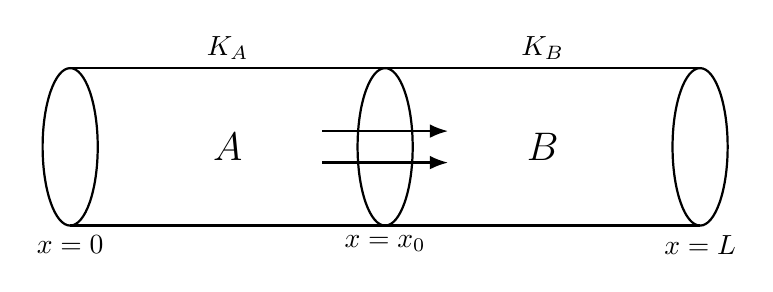
\begin{tikzpicture}[>=Latex, thick]

    % Parameters
    \def\L{8}
    \def\H{2}
    \def\xo{4}

    % Main cylinder body
    \draw (0,0) -- (\L,0);
    \draw (0,\H) -- (\L,\H);

    % Left ellipse
    \draw (0,\H/2) ellipse (0.35 and \H/2);

    % Middle divider
    \draw (\xo,\H/2) ellipse (0.35 and \H/2);

    % Right ellipse
    \draw (\L,\H/2) ellipse (0.35 and \H/2);

    % Labels inside
    \node at (2,\H/2) {\Large $A$};
    \node at (6,\H/2) {\Large $B$};

    % Region labels
    \node at (2,\H+0.25) {$K_A$};
    \node at (6,\H+0.25) {$K_B$};

    % Arrows at interface
    \draw[->] (\xo-0.8,1.2) -- (\xo+0.8,1.2);
    \draw[->] (\xo-0.8,0.8) -- (\xo+0.8,0.8);

    % x-axis labels
    \node[below] at (0,0) {$x=0$};
    \node[below] at (\xo,0) {$x=x_0$};
    \node[below] at (\L,0) {$x=L$};

\end{tikzpicture}
\end{center}

Some physical insights we must draw: firstly, for there to be no loss of heat energy, the \textbf{thermal energy fluxes at the threshold must be equal in magnitude}, for if they were not, heat energy would either accrue or diminish at \( x = x_{0} \), violating the conservation assumption. There is no addition or subtraction of thermal energy from the outside environment. Secondly, the fluxes must be identical in \textbf{direction}, as otherwise we would violate the premise that heat energy propagates from high to cold temperatures. In other words, \textbf{the fluxes across \( \pmb{A} \) and \( \pmb{B} \) are equal} in the limit as \( x_{0}-,x_{0}+ \rightarrow x_{0} \).
\[
	\phi_{A}\!\left( x_{0}-,t \right) = \phi_{B}\!\left( x_{0}+,t \right) 
\]
Using the Fourier heat law and canceling the sign, we have
\[
	K_{A}\!\left( x_{0}- \right)\frac{\partial u_{A}}{\partial x}\!\left( x_{0}-,t \right) = K_{B}\!\left( x_{0}+ \right)\frac{\partial u_{B}}{\partial x}\!\left( x_{0}+,t \right) 
\]
which is our equation for imposing heat conservation at the junction of the rods. To further enforce continuity of the spatial derivative, we must have the partial derivatives equal to each other, which implies that it is only equality of the conductivity constants that leads to continuity of the spatial derivatives.
\[
	K_{A}\!\left( x_{0}- \right) = K_{B}\!\left( x_{0}+ \right) 
\]

% QUESTION 3
\qs{1.3.3}{Consider a bath containing a fluid of specific heat \( c_{f} \) and mass density \( \rho_{f} \) that surrounds the end \( x = L \) of a one-dimensional rod. Suppose that the bath is rapidly-stirred in a manner such that the bath temperature is approximately uniform throughout, equaling the temperature at \( x = L \), \( u \!\left( L,t \right) \). Assume that the bath is thermally insulated except at its perfect thermal contact with the rod, where the bath may be heated or cooled by the rod. Determine an equation for the temperature in the bath. (This will be a boundary condition at the end \( x = L \).) (\textit{Hint}: See Exercise 1.3.2.)}

Before we begin, it helps to illustrate the scenario. Consider a bath with volume \( V_{\text{bath}} \), and let the area of the contact between the rod and the bath be \( A \). The conceptual setup should look something like this:

\begin{center}
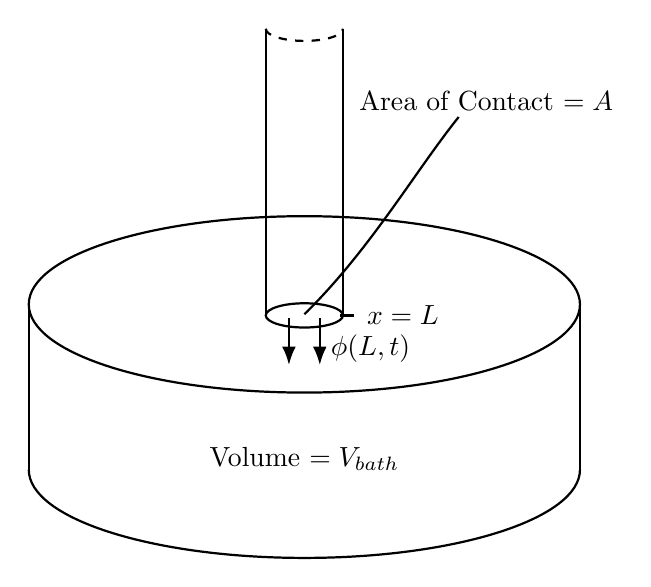
\begin{tikzpicture}[>=Latex, thick, scale=0.7]
    % ---- Parameters ----
    \def\bathRx{5}      % bath ellipse x-radius
    \def\bathRy{1.6}    % bath ellipse y-radius
    \def\bathH{3}       % bath height
    \def\rodRx{0.7}     % rod ellipse x-radius
    \def\rodRy{0.22}    % rod ellipse y-radius
    \def\rodTop{5.0}    % y of rod top
    \def\rodBot{-0.2}   % y of rod bottom (x=L face): below the bath rim
    % ---- Bath: side walls, bottom front arc, top ellipse ----
    \draw (-\bathRx,0) -- (-\bathRx,-\bathH);
    \draw (\bathRx,0) -- (\bathRx,-\bathH);
    \draw (-\bathRx,-\bathH) arc[start angle=180, end angle=360, x radius=\bathRx, y radius=\bathRy];
    % ---- Rod: vertical cylinder, end face submerged, centered on bath axis ----
    \draw (-\rodRx,\rodTop) -- (-\rodRx,\rodBot);
    \draw (\rodRx,\rodTop)  -- (\rodRx,\rodBot);
    % rod bottom face (x = L): full ellipse, drawn before bath top so the
    % bath rim overdraws the part of the rod that is inside the fluid
    \draw (0,\rodBot) ellipse[x radius=\rodRx, y radius=\rodRy];
    % ---- Bath top ellipse: drawn AFTER rod so the rim sits in front ----
    \draw (0,0) ellipse[x radius=\bathRx, y radius=\bathRy];
    % redraw the visible (above-rim) portion of the rod walls on top
    \draw (-\rodRx,\rodTop) -- (-\rodRx,0.12);
    \draw (\rodRx,\rodTop)  -- (\rodRx,0.12);
    % rod top (open): front arc dashed to suggest continuation
    \draw[dashed] (-\rodRx,\rodTop) arc[start angle=180, end angle=360, x radius=\rodRx, y radius=\rodRy];
    % ---- Labels and annotations ----
    % flux arrows: emanate from the submerged end face into the fluid
    \draw[->] (-0.28,\rodBot-0.05) -- (-0.28,\rodBot-0.9);
    \draw[->] (0.28,\rodBot-0.05)  -- (0.28,\rodBot-0.9);
    % phi label placed right next to the flux arrows
    \node at (1.2,\rodBot-0.6) {$\phi(L,t)$};
    % x = L label, pointing at the end face
    \node[right] at (\rodRx+0.25,\rodBot) {$x = L$};
    \draw (\rodRx+0.2,\rodBot) -- (\rodRx-0.05,\rodBot);
    % cross-sectional area A, leader curving in from the right
    \node at (3.3,3.7) {Area of Contact $= A$};
    \draw (2.8,3.4) .. controls (2.0,2.4) and (1.2,1.0) .. (0.0,\rodBot+0.02);
    % bath label, placed low and central in clear space
    \node at (0,-\bathH+0.2) {Volume $= V_{\text{bath}}$};
\end{tikzpicture}
\end{center}

With the given quantities, one natural first step might be to calculate the total energy of the bath as 
\[
	e \!\left( L,t \right) = c_{f}\rho_{f}V_{bath}u \!\left( L,t \right)
\]
Notice here \( e \) is defined in the textbook as an energy density, so we will make a slight alteration to that definition by multiplying through by the bath volume to express in terms of energy alone. Moreover, notice that this is an equation purely in terms of time \( t \). Differentiating with respect to time gives us
\[
	\frac{\partial e}{\partial t} = c_{f}\rho_{f}V_{\text{bath}}\frac{\partial u}{\partial t}\!\left( L,t \right) 
\]
From exercise 1.3.2, the physical intuition we are meant to derive is the insight that at the boundary \( x = L \), \textbf{the heat energy fluxes on either infinitesimal flank of the threshold \( \pmb{x = L} \) are equal}. 
\[
	\phi \!\left( L-,t \right) = \phi \!\left( L+,t \right)
\]
Originally, in deriving the heat equation, we considered a sub-section within a single rod, and identified a spatial gradient of the fluxes between the endpoints of that sub-section. In this case, we only have a \textit{singular} point of contact with an external source or sink (the rod), and thus we only have the flux \( \phi \) to concern ourselves with.

Being perspicacious with units, you will observe that \( \partial e / \partial t \) is in units of \( \text{W} \). However, the flux \( \phi \) is in units \( \text{W} / \text{m}^{2} \). One natural intuition to consider is the geometry of the rod is relevant, and particularly the area of the cross-sectional slice of the rod that touches the bath. Then
\[
	\phi \!\left( L,t \right)A = -K_{0} \frac{\partial u \!\left( L,t \right)}{\partial x}A
\]
Specifically, due to energy conservation, the only contribution or subtraction of the total heat energy in the bath will be due to the exchange of heat energy, or the flux, over the perfect thermal contact. Ergo, our final equation is
\[
	\frac{\partial e}{\partial t} = c_{f}\rho_{f}V_{\text{bath}}\frac{\partial u \!\left( L,t \right)}{\partial t} = -K_{0}\frac{\partial u \!\left( L,t \right)}{\partial x}A
\]
Conceptually, suppose the temperature of the bath increases with time. Then the initial temperature of the rod is warmer than that of the bath, and \( \partial u / \partial x < 0 \) corresponds to \( \partial u / \partial t > 0 \). Vice-versa, if \( \partial u / \partial t < 0 \)--temperature of the bath drops over time--then the rod is relatively cooler than the bath, and heat energy moves in the opposite direction.

\newpage
\subsection{\textsf{1.4 - Equilibrium Temperature Distribution}}
% QUESTION 1
\qs{1.4.1}{Determine the equilibrium temperature distribution for a one-dimensional rod with constant thermal properties with the following sources and boundary conditions:
\begin{enumerate}[label=(\alph*)]
	\item \( Q = 0 \), \quad \( u \!\left( 0 \right) = 0 \), \quad \( u \!\left( L \right) = T \)
	\item \( Q = 0 \), \quad \( u \!\left( 0 \right) = T \), \quad \( u \!\left( L \right) = 0 \)
	\item \( Q = 0 \), \quad \( \displaystyle{\frac{\partial u}{\partial x}\!\left( 0 \right) = 0} \), \quad \( u \!\left( L \right) = T \)
	\item \( Q = 0 \), \quad \( u \!\left( 0 \right) = T \), \quad \( \displaystyle{\frac{\partial u}{\partial x}\!\left( L \right) = \alpha} \)
	\item \( \displaystyle{\frac{Q}{K_{0}} = 1} \), \quad \( u \!\left( 0 \right) = T_{1} \), \quad \( u \!\left( L \right) = T_{2} \)
	\item \( \displaystyle{\frac{Q}{K_{0}} = x^{2}} \), \quad \( u \!\left( 0 \right) = T \), \quad \( \displaystyle{\frac{\partial u}{\partial x}\!\left( L \right) = 0} \)
	\item \( Q = 0 \), \quad \( u \!\left( 0 \right) = T \), \quad %
	\( \displaystyle{\frac{\partial u}{\partial x}\!\left( L \right) + u \!\left( L \right) = 0} \)
	\item \( Q = 0 \), \quad \( \displaystyle{\frac{\partial u}{\partial x}\!\left( 0 \right) - \!\left[ u \!\left( 0 \right) - T \right] = 0} \), \quad \( \displaystyle{\frac{\partial u}{\partial x}\!\left( L \right) = \alpha} \)
\end{enumerate}
In these you may assume that \( u \!\left( x,0 \right) = f \!\left( x \right) \).}

\begin{enumerate}[label=(\alph*)]
	\item No source, so we satisfy \( d^{2}u / dx^{2} = 0 \) and derive \( u \!\left( x \right) = C_{1}x + C_{2} \). The boundary conditions imply
	\begin{align*}
		u \!\left( 0 \right) & = C_{2} = 0 \\
		u \!\left( L \right) & = C_{1}L = T
	\end{align*}
	Leading us to equilibrium temperature distribution \( \displaystyle{u \!\left( x \right) = \frac{T}{L}x} \).
	\item Flip the boundary conditions from the previous exercise, and find
	\begin{align*}
		u \!\left( 0 \right) & = C_{2} = T \\
		u \!\left( L \right) & = C_{1}L + C_{2} = 0 \\ 
		      \implies C_{1} & = -\frac{T}{L}
	\end{align*}
	The equilibrium temperature distribution is \( \displaystyle{u \!\left( x \right) = -\frac{T}{L}x + T} \).
	\item We have the same temperature function \( u \!\left( x \right) = C_{1}x + C_{2} \), but this time with a first derivative boundary condition. Derive
	\begin{align*}
		\frac{\partial u}{\partial x}\!\left( 0 \right) & = C_{1} = 0 \\
		u \!\left( L \right) & = C_{2} = T
	\end{align*}
	Leaving us with \( u \!\left( x \right) = T \). Intuitively, this is correct because to have a zero spatial derivative at one end for a linear temperature distribution immediately implies a horizontal function.
	\item Once more, \( u \!\left( x \right) = C_{1}x + C_{2} \). We can intuitively infer that the line will have slope \( \alpha \) and intercept \( T \) at \( x = 0 \). Applying the boundary conditions gives us
	\begin{align*}
		u \!\left( 0 \right) & = C_{2} = T \\
		\frac{\partial u}{\partial x}\!\left( L \right) & = C_{1} = \alpha
	\end{align*}
	Leading us to \( u \!\left( x \right) = \alpha x + T \). Our intuition proved correct for this simple case, but it is a lesson in examining how the nature of internal sources or boundary conditions can influence the shape of the equilibrium temperature distribution.
	\item Now, our source is non-zero. Setting \( \partial u / \partial t = 0 \), we have
	\[
		K_{0}\frac{d^{2}u}{dx^{2}} + K_{0} = 0
	\]
	Divide through by \( K_{0} \) and isolate the second derivative to get
	\[
		\frac{d^{2}u}{dx^{2}} = -1
	\]
	Integrating twice yields the quadratic
	\[
		u \!\left( x \right) = -\frac{x^{2}}{2} + C_{1}x + C_{2} 
	\]
	Imposing the boundary conditions, derive
	\begin{align*}
		u \!\left( 0 \right) & = C_{2} = T_{1} \\
		u \!\left( L \right) & = -\frac{L^{2}}{2} + C_{1}L + T_{1} = T_{2} \\ 
		      \implies C_{1} & = \frac{2 \!\left( T_{2} - T_{1} \right) + L^{2}}{2L}
	\end{align*}
	Leaving us with
	\[
		u \!\left( x \right) = -\frac{x^{2}}{2} + \!\left[ \frac{2 \!\left( T_{2} - T_{1} \right) + L^{2}}{2L} \right]x + T_{1} 
	\]
	\item From
	\[
		K_{0}\frac{d^{2}u}{dx^{2}} + K_{0}x^{2} = 0 
	\]
	Derive
	\[
		u \!\left( x \right) = -\frac{x^{4}}{12} + C_{1}x + C_{2} 
	\]
	And apply boundary conditions
	\begin{align*}
		u \!\left( 0 \right) & = C_{2} = T \\
		\frac{\partial u}{\partial x}\!\left( L \right) & = -\frac{L^{3}}{3} + C_{1} = 0 \\
		\implies C_{1} & = \frac{L^{3}}{3}
	\end{align*}
	Finishing with temperature distribution
	\[
		u \!\left( x \right) = -\frac{x^{4}}{12} + \frac{L^{3}}{3}x + T
	\]
	\item Returning again to the form \( u \!\left( x \right) = C_{1}x + C_{2} \), apply boundary conditions
	\begin{align*}
		u \!\left( 0 \right) & = C_{2} = T \\
		\frac{\partial u}{\partial x}\!\left( L \right) + u \!\left( L \right) & = C_{1}\!\left( 1 + L \right) + T = 0 \\ 
		C_{1} & = -\frac{T}{1 + L}
	\end{align*}
	Leading to
	\[
		u \!\left( x \right) = T \!\left( 1 - \frac{x}{1 + L} \right) 
	\]
	\item Lastly, we finish up this set with, once more, temperature distribution form \( u \!\left( x \right) = C_{1}x + C_{2} \). Applying the boundary conditions gives us coefficients
	\begin{align*}
		\frac{\partial u}{\partial x}\!\left( 0 \right) - \!\left[ u \!\left( 0 \right) - T \right] & = C_{1} - C_{2} + T = 0 \\
		\frac{\partial u}{\partial x}\!\left( L \right) & = C_{1} = \alpha \\ 
		\implies C_{2} & = \alpha + T
	\end{align*}
	and concluding with
	\[
		u \!\left( x \right) = \alpha \!\left( x + 1 \right) + T 
	\]
\end{enumerate}

\newpage
% QUESTION 2
\qs{1.4.2}{Consider the equilibrium temperature distribution for a uniform one-dimensional rod with sources \( Q / K_{0} = x \) of thermal energy, subject to the boundary conditions \( u \!\left( 0 \right) = 0 \) and \( u \!\left( L \right) = 0 \).
\begin{enumerate}[label=(\alph*)]
	\item Determine the heat energy generated per unit time inside the entire rod.
	\item Determine the heat energy flowing out of the rod per unit time at \( x = 0 \) and at \( x = L \).
	\item What relationships should exist between the answers in parts (a) and (b)? 
\end{enumerate}}

\begin{enumerate}[label=(\alph*)]
	\item Conceptually, we have to consider \( Q / K_{0} = x \) as a \textbf{distributed source} of thermal energy, whilst the problem asks about the rate of heat energy generation \textbf{for the entire rod}. Recall that \( Q \) itself is a measure of heat energy per unit volume per unit time. Therefore, the problem entails summing over all of these distributed sources of heat energy internal to the rod, or
	\[
		Q_{\text{total}} = \int^{L}_{0} Q \, dx = K_{0}\int^{L}_{0} x \, dx = \frac{K_{0}L^{2}}{2} 
	\]
	\item The objective here is to calculate the fluxes \( -K_{0} \partial u / \partial x \) at the boundaries. Derive the equilibrium temperature distribution from 
	\[
		K_{0}\frac{d^{2}u}{dx^{2}} + K_{0}x = 0 \quad \implies \quad u \!\left( x \right) = -\frac{x^{3}}{6} + C_{1}x + C_{2} 
	\]
	where applying boundary conditions yields \( u \!\left( 0 \right) = C_{2} = 0 \) and \( u \!\left( L \right) = -L^{3} / 6 + C_{1}L = 0 \), or \( C_{1} = L^{2} / 6 \). Then our function is
	\[
		u \!\left( x \right) = -\frac{x^{3}}{6} + \frac{L^{2}}{6}x 
	\]
	which has spatial derivative
	\[
		\frac{\partial u}{\partial x} = -\frac{x^{2}}{2} + \frac{L^{2}}{6} 
	\]
	The fluxes are then
	\begin{align*}
		\phi \!\left( 0,t \right) & = -K_{0}\frac{\partial u}{\partial x}\!\left( 0,t \right) = -\frac{K_{0}L^{2}}{6} \\
		\phi \!\left( L,t \right) & = -K_{0}\frac{\partial u}{\partial x}\!\left( L,t \right) = K_{0} \frac{L^{2}}{3}
	\end{align*}
	And since \( K_{0} > 0 \), the directionality of the fluxes is clear. Heat energy propagates leftward at \( x = 0 \) and rightward at \( x = L \). Thus at both ends, \textbf{energy leaves the rod}.
	Now, taking a step back, consider the flux component of the heat equation, which gives us the combined heat energy outflow per unit time at \textit{both} boundaries.
	\[
		-\int^{L}_{0} \frac{\partial \phi}{\partial x} \, dx = K_{0}\frac{\partial u}{\partial x}\!\left( L,t \right) - K_{0}\frac{\partial u}{\partial x}\!\left( 0,t \right) = -\frac{K_{0}L^{2}}{2}
	\]
	\item Returning to the key physical premise of the problem: that we are at \textbf{equilibrium state} for temperature, definitionally we know that \( \partial u / \partial t = 0 \). Equivalently, \( \partial e / \partial t = 0 \). \textbf{We can then deduce for the entire bar}
	\[
		\frac{\partial }{\partial t}\int^{L}_{0} e \, dx = -\int^{L}_{0} \frac{\partial \phi}{\partial x} \, dx + Q_{\text{total}} = 0
	\]
	By conservation of heat energy within the rod, the rate of internal heat energy generation must match the rate of outflow at the boundaries. Indeed, we can confirm
	\[
		\frac{\partial }{\partial t}\int^{L}_{0} e \, dx = -\int^{L}_{0} \frac{\partial \phi}{\partial x} \, dx + Q_{\text{total}} = -\frac{K_{0}L^{2}}{2} + \frac{K_{0}L^{2}}{2} = 0
	\]
\end{enumerate}

% QUESTION 3
\qs{1.4.3}{Determine the equilibrium temperature distribution for a one-dimensional rod composed of two different materials in perfect thermal contact at \( x = 1 \). For \( 0 < x < 1 \), there is one material (\( c \rho = 1 \), \( K_{0} = 1 \)) with a constant source (\( Q = 1 \)), whereas for the other \( 1 < x < 2 \), there are no sources (\( Q = 0 \), \( c \rho = 2 \), \( K_{0} = 2 \)) (see Exercise 1.3.2) with \( u \!\left( 0 \right) = 0 \) and \( u \!\left( 2 \right) = 0 \).}

By the assumption of perfect thermal contact, we know that 

\begin{enumerate}[label=(\alph*)]
	\item the temperatures at the boundary must be equal:
	\[
		u_{A}\!\left( 1-,t \right) = u_{B}\!\left( 1+,t \right) 
	\]
	\item the fluxes at the boundary are equal: 
	\[ 
		\phi_{A}\!\left( 1-,t \right) = \phi_{B}\!\left( 1+,t \right) 
	\]
\end{enumerate}

\begin{center}
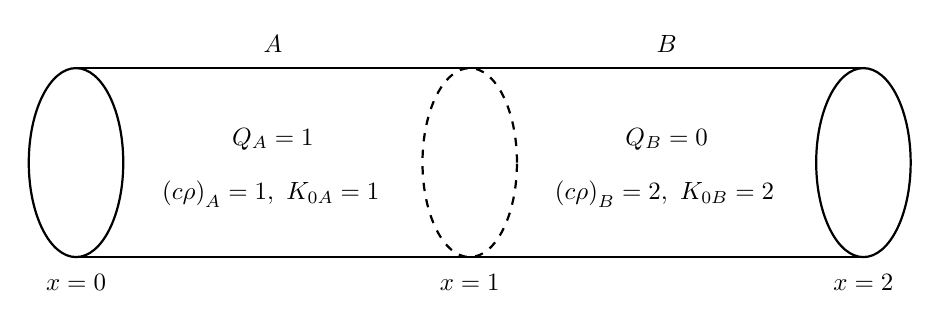
\begin{tikzpicture}[thick, every node/.style={scale=0.9}]

% --- Segment A (x=0 to x=1) ---
\draw (-1,0) ellipse (0.6cm and 1.2cm);
\draw (-1, 1.2) -- (4.0, 1.2);
\draw (-1,-1.2) -- (4.0,-1.2);
\draw[dashed] (4.0, 0) ellipse (0.6cm and 1.2cm);
\node at (1.5, 0.3) {$Q_{A} = 1$};
\node at (1.5, -0.4) {$\!\left( c\rho \right)_{A}=1,\ K_{0A}=1$};
\node at (1.5, 1.5) {$A$};
\node[below] at (-1, -1.3) {$x=0$};
\node[below] at (4.0, -1.3) {$x=1$};

% --- Segment B (x=1 to x=2) ---
\draw (4.0, 1.2) -- (9.0, 1.2);
\draw (4.0,-1.2) -- (9.0,-1.2);
\draw (9.0, 0) ellipse (0.6cm and 1.2cm);
\node at (6.5, 0.3) {$Q_{B} = 0$};
\node at (6.5, -0.4) {$\!\left( c\rho \right)_{B}=2,\ K_{0B}=2$};
\node at (6.5, 1.5) {$B$};
\node[below] at (9.0, -1.3) {$x=2$};

\end{tikzpicture}%
\end{center}

First, let us derive the temperature distributions for sections \( A \) and \( B \) to the extent that we can. In \( A \), we have
\[
	K_{0A}\frac{d^{2}u_{A}}{dx^{2}} + 1 = 0 
\]
Isolating the second derivative and integrating twice, derive
\[
	u_{A}\!\left( x \right) = -\frac{x^{2}}{2} + C_{1A}x + C_{2A}  
\]
Now, from the boundary condition \( u_{A}\!\left( 0 \right) = 0 \), we immediately deduce \( C_{2A} = 0 \), so now we are left with
\[
	u_{A}\!\left( x \right) = -\frac{x^{2}}{2} + C_{1A}x  
\]
Moving onto section \( B \), we have
\[
	\frac{d^{2}u_{B}}{dx^{2}} = 0
\]
which yields
\[
	u_{B}\!\left( x \right) = C_{1B}x + C_{2B}
\]
Imposing the second boundary condition, we can further conclude
\[
	u_{B}\!\left( 2 \right) = 2C_{1B} + C_{2B} = 0 \quad \implies \quad C_{2B} = -2C_{1B}, \quad u_{B}\!\left( x \right) = C_{1B}\!\left( x - 2 \right)
\]
The last component we need is the fluxes, and thus spatial derivatives for both sections, which are
\begin{align*}
	K_{0A}\frac{\partial u_{A}}{\partial x} & = -x + C_{1A} \\
	K_{0B}\frac{\partial u_{B}}{\partial x} & = 2C_{1B}
\end{align*}
Finally, we may apply boundary conditions (a) and (b) at \( x = 1 \).
\begin{alignat*}{5}
	u_{A}\!\left( 1-,t \right) & = -\frac{1}{2} && + C_{1A} && = - && C_{1B} && = u_{B}\!\left( 1+,t \right) \\
	K_{0A}\frac{\partial u_{A}}{\partial x}\!\left( 1-,t \right) & = -1 && + C_{1A} && = && 2C_{1B} && = K_{0B}\frac{\partial u_{B}}{\partial x}\!\left( 1+,t \right)
\end{alignat*}
Solve for this using matrix algebra, using which we find
\[
	C_{1A} = \frac{2}{3}, \quad C_{1B} = -\frac{1}{6}, \quad C_{2B} = \frac{1}{3} 
\]
Giving us equilibrium temperature distribution
\[
	u \!\left( x \right) = \begin{cases}
		\displaystyle{-\frac{x^{2}}{2} + \frac{2}{3}x}, & 0 < x < 1 \\[12pt]
		\displaystyle{-\frac{x}{6} + \frac{1}{3}}, & 1 < x < 2 \\
	\end{cases} 
\]
Observe that \( c \rho \) were irrelevant to this problem, as they matter only in the transient, not equilibrium state.

\vspace{12pt}

% QUESTION 4
\qs{1.4.4}{If both ends of a rod are insulated, derive \textit{from the partial differential equation} that the total thermal energy in the rod is constant.}

By the insulation assumption, we must have
\[
	\frac{\partial u}{\partial x}\!\left( 0,t \right) = \frac{\partial u}{\partial x}\!\left( L,t \right) = 0 
\]
Suppose further that \( u \!\left( x,0 \right) = f \!\left( x \right) \), and \( c \) and \( \rho \) the specific heat and density, respectively. Consider the integral conservation equation
\[
	\frac{d }{d t}\underbrace{\int^{L}_{0} e \, dx}_{\substack{\text{total thermal} \\ \text{energy}}} = \frac{d }{d t}\int^{L}_{0} c \rho u \!\left( x,t \right) \, dx = -\int^{L}_{0} \frac{\partial \phi}{\partial x} \, dx = K_{0}\frac{\partial u}{\partial x}\!\left( L,t \right) - K_{0}\frac{\partial u}{\partial x}\!\left( 0,t \right) = 0
\]
Since the derivative of the total energy density is zero, we may deduce that it is constant.

\vspace{12pt}

% QUESTION 5
\qs{1.4.5}{Consider a one-dimensional rod \( 0 \le x \le L \) of known length and known constant thermal properties without sources. Suppose that the temperature is an \textit{unknown} constant \( T \) at \( x = L \). Determine \( T \) if we know (in the steady state) both the temperature and the heat flow at \( x = 0 \).}

Let \( u \!\left( 0 \right) = T_{1} \) and \( \partial u / \partial x \!\left( 0 \right) \) be known quantities. Since the rod is bereft of internal heat sources, the steady state temperature distribution is of form \( u \!\left( x \right) = C_{1}x + C_{2} \). From the boundary conditions, \( u \!\left( 0 \right) = C_{2} = T_{1} \) and \( \partial u / \partial x \!\left( 0 \right) = C_{1} \). Then \( u \!\left( L \right) \) is
\[
	u \!\left( L \right) = \frac{\partial u}{\partial x}\!\left( 0 \right)L + T_{1}
\]

% QUESTION 6
\qs{1.4.6}{The two ends of a uniform rod of length \( L \) are insulated. There is a constant source of thermal energy \( Q_{0} \neq 0 \), and the temperature is initially \( u \!\left( x,0 \right) = f \!\left( x \right) \).
\begin{enumerate}[label=(\alph*)]
	\item Show mathematically that there does not exist any equilibrium temperature distribution. Briefly explain physically.
	\item Calculate the total thermal energy in the entire rod.
\end{enumerate}}

\begin{enumerate}[label=(\alph*)]
	\item Since insulation implies there is no heat energy flux at the rod's boundaries, the integral conservation equation reduces to
	\[
		\frac{d }{dt}\int^{L}_{0} c \rho u \, dx = \int^{L}_{0} Q_{0} \, dx = Q_{0}L \neq 0
	\]
	which implies that the rate of change of the total thermal energy is never zero. To deduce that we also cannot have \( \partial u / \partial t = 0 \), suppose otherwise. Then \( \partial u / \partial t = 0 \) implies
	\[
		\int^{L}_{0} c \rho \frac{\partial u}{\partial t} \, dx = 0  
	\]
	which immediately contradicts our result. Thus this precludes the existence of an equilibrium temperature distribution.
	\item Integrating from time \( 0 \) to \( t \) and using the dummy variable \( T \), derive
	\begin{align*}		
		\int^{t}_{0} \!\left[ \frac{d }{dT}\int^{L}_{0} c \rho u \!\left( x,T \right) \, dx \right] \, dT & = \int^{t}_{0} \!\left[ \int^{L}_{0} Q_{0} \, dx \right] \, dT \\
		\int^{L}_{0} c \rho u \!\left( x,t \right) \, dx & = \underbrace{\int^{L}_{0} c \rho f \!\left( x \right) \, dx}_{\text{initial thermal energy}} + \underbrace{Q_{0}Lt}_{\text{internal source}}
	\end{align*}
	where we make the substitution \( u \!\left( x,0 \right) = f \!\left( x \right) \). Intuitively, the total thermal energy is a sum of the initial thermal energy and the energy contributed by the heat source over time.
\end{enumerate}

% QUESTION 7
\qs{1.4.7}{For the following problems, determine an equilibrium temperature distribution (if one exists). For what values of \( \beta \) are there solutions? Explain physically.
\begin{enumerate}[label=(\alph*)]
	\item \( \displaystyle{\frac{\partial u}{\partial t} = \frac{\partial^{2}u}{\partial x^{2}} + 1} \), \quad \( u \!\left( x,0 \right) = f \!\left( x \right) \), \quad \( \displaystyle{\frac{\partial u}{\partial x}\!\left( 0,t \right) = 1} \), \quad \( \displaystyle{\frac{\partial u}{\partial x}\!\left( L,t \right) = \beta} \)
	\item \( \displaystyle{\frac{\partial u}{\partial t} = \frac{\partial^{2}u}{\partial x^{2}}} \), \quad \( u \!\left( x,0 \right) = f \!\left( x \right) \), \quad \( \displaystyle{\frac{\partial u}{\partial x}\!\left( 0,t \right) = 1} \), \quad \( \displaystyle{\frac{\partial u}{\partial x}\!\left( L,t \right) = \beta} \)
	\item \( \displaystyle{\frac{\partial u}{\partial t} = \frac{\partial^{2}u}{\partial x^{2}} + x - \beta} \), \quad \( u \!\left( x,0 \right) = f \!\left( x \right) \), \quad \( \displaystyle{\frac{\partial u}{\partial x}\!\left( 0,t \right) = 0} \), \quad \( \displaystyle{\frac{\partial u}{\partial x}\!\left( L,t \right) = 0} \)
\end{enumerate}}

\begin{enumerate}[label=(\alph*)]
	\item Proceed by letting \( \partial u / \partial t = 0 \) to see what becomes of this assumption. We have temperature distribution
	\[
		u \!\left( x \right) = -\frac{x^{2}}{2} + C_{1}x + C_{2} 
	\]
	which has spatial derivative \( \partial u / \partial x = -x + C_{1} \). Then \( \partial u / \partial x \!\left( 0,t \right) = C_{1} = 1 \) and \( \partial u / \partial x \!\left( L,t \right) = 1 - L = \beta \); this is the only permissible value of \( \beta \) for an equilibrium to exist. Unfortunately, we are at a dead end for identifying \( C_{2} \), but this merely sets the vertical position of the equilibrium temperature distribution and can be determined if prescribed temperatures at the ends are given.
	\item Let \( \partial u / \partial t = 0 \). No source, so our temperature distribution is
	\[
		u \!\left( x \right) = C_{1}x + C_{2} 
	\]
	and spatial derivative \( \partial u / \partial x = C_{1} \). Since this is not a function of \( x \) and is constant throughout the rod, the boundary conditions at either end must be equal, so we must have \( C_{1} = \beta = 1 \) for an equilibrium to exist. Again, we have a situation in which \( C_{2} \) cannot be determined, but prescribing temperatures at the boundaries rectifies this.
	\item Let \( \partial u / \partial t = 0 \). Incorporating the distributed heat source, we have temperature distribution
	\[
		u \!\left( x \right) = -\frac{x^{3}}{6} + \frac{\beta x^{2}}{2} + C_{1}x + C_{2} 
	\]
	Then our spatial derivative is 
	\[
		\frac{\partial u}{\partial x} = -\frac{x^{2}}{2} + \beta x + C_{1} 
	\]
	Evaluating at the ends, we get \( \partial u / \partial x \!\left( 0,t \right) = C_{1} = 0 \) and \( \partial u / \partial x \!\left( L,t \right) = \beta L - L^{2} / 2 = 0 \), implying that \( \beta = L / 2 \) for the equilibrium state.
\end{enumerate}

% QUESTION 8
\qs{1.4.8}{Express the integral conservation law for the entire rod with constant thermal properties. Assume the heat flow is known to be different constants at both ends. By integrating with respect to time, determine the total thermal energy in the rod. (Hint: Use the initial condition.)
\begin{enumerate}[label=(\alph*)]
	\item Assume there are no sources.
	\item Assume the sources of thermal energy are constant.
\end{enumerate}}

In both cases, let the initial condition be \( u \!\left( x,0 \right) = f \!\left( x \right) \). Let \( \phi \!\left( 0,t \right) = \alpha \) and \( \phi \!\left( L,t \right) = \beta \).

\begin{enumerate}[label=(\alph*)]
	\item \begin{align*}
			\frac{d }{dt}\int^{L}_{0} c \rho u \, dx & = -\int^{L}_{0} \frac{\partial \phi}{\partial x} \, dx \\
								 & = \phi \!\left( 0,t \right) - \phi \!\left( L,t \right) \\
								 & = \alpha - \beta
	\end{align*}
	Integrate from time \( 0 \) to \( t \) to get
	\begin{alignat*}{2}
		&& \int^{t}_{0} \!\left[ \frac{d }{dT} \int^{L}_{0} c \rho u \!\left( x,T \right) \, dx \right] \, dT & = \int^{t}_{0} \!\left( \alpha - \beta \right) \, dT \\
		\implies && \int^{L}_{0} c \rho u \!\left( x,t \right) \, dx & = \int^{L}_{0} c \rho f \!\left( x \right) \, dx + \!\left( \alpha - \beta \right)t  
	\end{alignat*}
	\item 
	\begin{align*}
		\frac{d }{dt}\int^{L}_{0} c \rho u \, dx & = -\int^{L}_{0} \frac{\partial \phi}{\partial x} \, dx + \int^{L}_{0} Q \, dx \\
							 & = \phi \!\left( 0,t \right) - \phi \!\left( L,t \right) + QL \\
							 & = \alpha - \beta + QL
	\end{align*}
	Integrate from time \( 0 \) to \( t \) to get
	\begin{alignat*}{2}
		&& \int^{t}_{0} \!\left[ \frac{d }{dT}\int^{L}_{0} c \rho u \!\left( x,T \right) \, dx \right] \, dT & = \int^{t}_{0} \!\left( \alpha - \beta + QL \right) \, dT  \\
		\implies && \int^{L}_{0} c \rho u \!\left( x,t \right) \, dx & = \int^{L}_{0} c \rho f \!\left( x \right) \, dx + \!\left( \alpha - \beta + QL \right)t
	\end{alignat*}
\end{enumerate}

% QUESTION 9
\qs{1.4.9}{Derive the integral conservation law for the entire rod with constant thermal properties by integrating the heat equation (1.2.10) (assuming no sources). Show the result is equivalent to (1.2.4).}

The heat equation is
\[
	\frac{\partial u}{\partial t} = k \frac{\partial^{2}u}{\partial x^{2}} 
\]
where \( k = K_{0} / c \rho \). Multiply through by \( c \rho \) and integrate with respect to \( x \) over \( a \le x \le b \) to get
\begin{align*}
	\int^{b}_{a} c \rho \frac{\partial u}{\partial t} \, dx & = K_{0}\int^{b}_{a} \frac{\partial^{2}u}{\partial x^{2}} \, dx \\
								& = K_{0}\!\left[ \frac{\partial u}{\partial x}\!\left( b,t \right) - \frac{\partial u}{\partial x}\!\left( a,t \right) \right] \\
								& = \phi \!\left( a,t \right) - \phi \!\left( b,t \right)
 \end{align*}
By Leibniz's rule, we can pull the differential operator out of the integral. We restore the integral conservation law:
\[
	\frac{d }{dt}\int^{b}_{a} c \rho u \, dx = \phi \!\left( a,t \right) - \phi \!\left( b,t \right)
\]

% QUESTION 10
\qs{1.4.10}{Suppose \( \frac{\partial u}{\partial t} = \frac{\partial^{2}u}{\partial x^{2}} + 4 \), \( u \!\left( x,0 \right) = f \!\left( x \right) \), \( \frac{\partial u}{\partial x}\!\left( 0,t \right) = 5 \), \( \frac{\partial u}{\partial x}\!\left( L,t \right) = 6 \). Calculate the total thermal energy in the one-dimensional rod (as a function of time).}

By the integral conservation law,
\begin{align*}
	\frac{d }{dt}\int^{L}_{0} c \rho u \, dx & = \frac{\partial u}{\partial x}\!\left( L,t \right) - \frac{\partial u}{\partial x}\!\left( 0,t \right) + \int^{L}_{0} 4 \, dx \\
						 & = 6 - 5 + 4L \\
						 & = 1 + 4L
\end{align*}
Integrate from time \( 0 \) to \( t \) to get
\begin{alignat*}{2}
	&& \int^{t}_{0} \!\left[ \frac{d }{dT} \int^{L}_{0} c \rho u \!\left( x,T \right) \, dx \right] \, dT & = \int^{t}_{0} \!\left( 1 + 4L \right) \, dT \\
	\implies && \int^{L}_{0} c \rho u \!\left( x,t \right) \, dx & = \int^{L}_{0} c \rho f \!\left( x \right) \, dx + \!\left( 1 + 4L \right)t \\ 
\end{alignat*}

% QUESTION 11
\qs{1.4.11}{Suppose \( \frac{\partial u}{\partial t} = \frac{\partial^{2}u}{\partial x^{2}} + x \), \( u \!\left( x,0 \right) = f \!\left( x \right) \), \( \frac{\partial u}{\partial x}\!\left( 0,t \right) = \beta \), \( \frac{\partial u}{\partial x}\!\left( L,t \right) = 7 \).
\begin{enumerate}[label=(\alph*)]
	\item Calculate the total thermal energy in the one-dimensional rod (as a function of time).
	\item From part (a), determine the value of \( \beta \) for which an equilibrium exists. For this value of \( \beta \), determine \( \lim\limits_{t \to \infty} u \!\left( x,t \right) \).
\end{enumerate}}

\begin{enumerate}[label=(\alph*)]
	\item By the integral conservation law,
	\begin{align*}
		\frac{d }{dt}\int^{L}_{0} c \rho u \, dx & = \frac{\partial u}{\partial x}\!\left( L,t \right) - \frac{\partial u}{\partial x}\!\left( 0,t \right) + \int^{L}_{0} x \, dx \\
		 & = 7 - \beta + \frac{L^{2}}{2}
	\end{align*}
	Integrating over time from \( 0 \) to \( t \), derive
	\begin{alignat*}{2}
		 && \int^{t}_{0} \!\left[ \frac{d }{dT}\int^{L}_{0} c \rho u \!\left( x,T \right)\, dx \right] \, dT & = \int^{t}_{0} \!\left( 7 - \beta + \frac{L^{2}}{2} \right) \, dT \\
		\implies && \int^{L}_{0} c \rho u \!\left( x,t \right) \, dx & = \int^{L}_{0} c \rho f \!\left( x \right) \, dx + \!\left( 7 - \beta + \frac{L^{2}}{2} \right)t
	\end{alignat*}
	\item Let \( \partial u / \partial t = 0 \). Then
	\[
		u \!\left( x \right) = -\frac{x^{3}}{6} + C_{1}x + C_{2} 
	\]
	with spatial derivative
	\[
		\frac{\partial u}{\partial x} = -\frac{x^{2}}{2} + C_{1} 
	\]
	Applying the boundary conditions, we have
	\begin{align*}
		\frac{\partial u}{\partial x}\!\left( 0,t \right) & = C_{1} = \beta \\
		\frac{\partial u}{\partial x}\!\left( L,t \right) & = \beta - \frac{L^{2}}{2} = 7 \\ 
		\beta & = 7 + \frac{L^{2}}{2}
	\end{align*}
	Then in the steady-state, the temperature distribution is
	\[
		\lim\limits_{t \to \infty} u \!\left( x,t \right) = u \!\left( x \right) = -\frac{x^{3}}{6} + \!\left( 7 + \frac{L^{2}}{2} \right)x + C_{2} 
	\]
	Where \( C_{2} \) is an arbitrary constant dependent on the initial condition.
\end{enumerate}

% QUESTION 12
\qs{1.4.12}{Suppose the concentration \( u \!\left( x,t \right) \) of a chemical satisfies Fick's law (1.2.13), and the initial concentration is given as \( u \!\left( x,0 \right) = f \!\left( x \right) \). Consider a region \( 0 < x < L \) in which the flow is specified at both ends \( -k \frac{\partial u}{\partial x}\!\left( 0,t \right) = \alpha \) and \( -k \frac{\partial u}{\partial x}\!\left( L,t \right) = \beta \). Assume \( \alpha \) and \( \beta \) are constants.
\begin{enumerate}[label=(\alph*)]
	\item Express the conservation law for the entire region.
	\item Determine the total amount of chemical in the region as a function of time (using the initial condition).
	\item Under what conditions is there an equilibrium chemical concentration, and what is it?
\end{enumerate}}

\begin{enumerate}[label=(\alph*)]
	\item \[
		\frac{d }{dt}\int^{L}_{0} u \, dx = -\int^{L}_{0} \frac{\partial \phi}{\partial x} \, dx = -k \!\left[ \frac{\partial u}{\partial x}\!\left( 0,t \right) - \frac{\partial u}{\partial x}\!\left( L,t \right) \right] = \alpha - \beta
	\]
	\item Since we define \( u \!\left( x,t \right) \) as the concentration of the chemical per unit volume, we will need to multiply through by the cross-sectional area of the rod \( A \). Integrate over time from \( 0 \) to \( t \) to get
	\begin{alignat*}{2}
		&& \int^{t}_{0} \!\left[ \frac{d }{dT}\int^{L}_{0} u \!\left( x,T \right)A \, dx  \right] \, dT & = A \int^{t}_{0} \!\left( \alpha - \beta \right) \, dT \\
		\implies && \int^{L}_{0} u \!\left( x,t \right)A \, dx & = A \!\left[ \int^{L}_{0} f \!\left( x \right) \, dx + \!\left( \alpha - \beta \right)t \right]
	\end{alignat*}
	\item Let \( \partial u / \partial t = 0 \). With zero sources, we have chemical concentration
	\[
		u \!\left( x \right) = C_{1}x + C_{2}
	\]
	Applying the boundary conditions, we have
	\[
		\frac{\partial u}{\partial x}\!\left( 0,t \right) = -\frac{\alpha}{k} = C_{1} = -\frac{\beta}{k} = \frac{\partial u}{\partial x}\!\left( L,t \right) 
	\]
	from which we can conclude that equilibrium exists only when \( \alpha = \beta \).
\end{enumerate}

\newpage
% QUESTION 13
\qs{1.4.13}{Do Exercise 1.4.12 if \( \alpha \) and \( \beta \) are functions of time.}

\begin{enumerate}[label=(\alph*)]
	\item Now we assume \( \alpha \) and \( \beta \) are functions of time, which changes the conservation equation to
	\[
		\frac{d }{dt}\int^{L}_{0} u \, dx = -\int^{L}_{0} \frac{\partial \phi}{\partial x} \, dx = -k \!\left[ \frac{\partial u}{\partial x}\!\left( 0,t \right) - \frac{\partial u}{\partial x}\!\left( L,t \right) \right] = \alpha \!\left( t \right) - \beta \!\left( t \right)
	\]
	\item Since \( \alpha \) and \( \beta \) are no longer pure constants, we can only consider their integrals in the abstract as part of the total amount of chemical.
	\[
		\int^{L}_{0} u \!\left( x,t \right)A \, dx = A \!\left[ \int^{L}_{0} f \!\left( x \right) \, dx + \int^{t}_{0} \!\left( \alpha \!\left( T \right) - \beta \!\left( T \right) \right) \, dT \right]  
	\]
	\item Lastly, by assuming \( \partial u / \partial t = 0 \) and that \( \lim\limits_{t \to \infty} u \!\left( x,t \right) = u \!\left( x \right) \), it still follows that \( C_{1} \) is a constant. From the boundary conditions, we still must have
	\[
		-\lim\limits_{t \to \infty}\frac{\alpha \!\left( t \right)}{k} = C_{1} = -\lim\limits_{t \to \infty}\frac{\beta \!\left( t \right)}{k} 
	\]
	In other words, \( \alpha \!\left( t \right) \) and \( \beta \!\left( t \right) \) must approach constants in the temporal limit for a steady-state to exist.
\end{enumerate}

\newpage
\subsection{\textsf{1.5 - Derivation of the Heat Equation in Two or Three Dimensions}}
% QUESTION 1
\qs{1.5.1}{Let \( c \!\left( x,y,z,t \right) \) denote the concentration of a pollutant (the amount per unit volume).
\begin{enumerate}[label=(\alph*)]
	\item What is an expression for the total amount of pollutant in the region \( R \)?
	\item Suppose that the flow \( \pmb{J} \) of the pollutant is proportional to the gradient of the concentration. (Is this reasonable?) Express conservation of the pollutant.
	\item Derive the partial differential equation governing the diffusion of the pollutant.
\end{enumerate}}

\begin{enumerate}[label=(\alph*)]
	\item \( \iiint_{R} c \, dV \)
	\item Let \( \pmb{J} = A \nabla c \). This is simply Fick's law in three dimensions when \( A = -k \).
	\[
		\pmb{J} = -k \nabla c \!\left( x,y,z,t \right) = \frac{\partial c}{\partial x}\pmb{\hat{i}} + \frac{\partial c}{\partial y}\pmb{\hat{j}} + \frac{\partial c}{\partial z}\pmb{\hat{k}}
	\]
	Conservation is when there is no change in mass in the volume, so assuming that the three-dimensional region is invariant with time, we have
	\[
		\frac{d }{dt}\iiint_{R} c \!\left( x,y,z,t \right) \, dV = 0 \quad \implies \quad \frac{\partial c}{\partial t} = 0 
	\]
	\item Conceptually, the rate of change of the amount of pollutant is expressed by
	\[
		\vcenter{\hbox{\shortstack{Rate of change\\of amount\\of pollutant}}}
		\quad=\quad
		\vcenter{\hbox{\shortstack{Surface flux\\of the pollutant\\per unit time}}}
		\quad+\quad
		\vcenter{\hbox{\shortstack{Internal pollutant\\generation\\per unit time}}}
	\]
	It is helpful to visualize the physics with a diagram:
	\begin{center}
	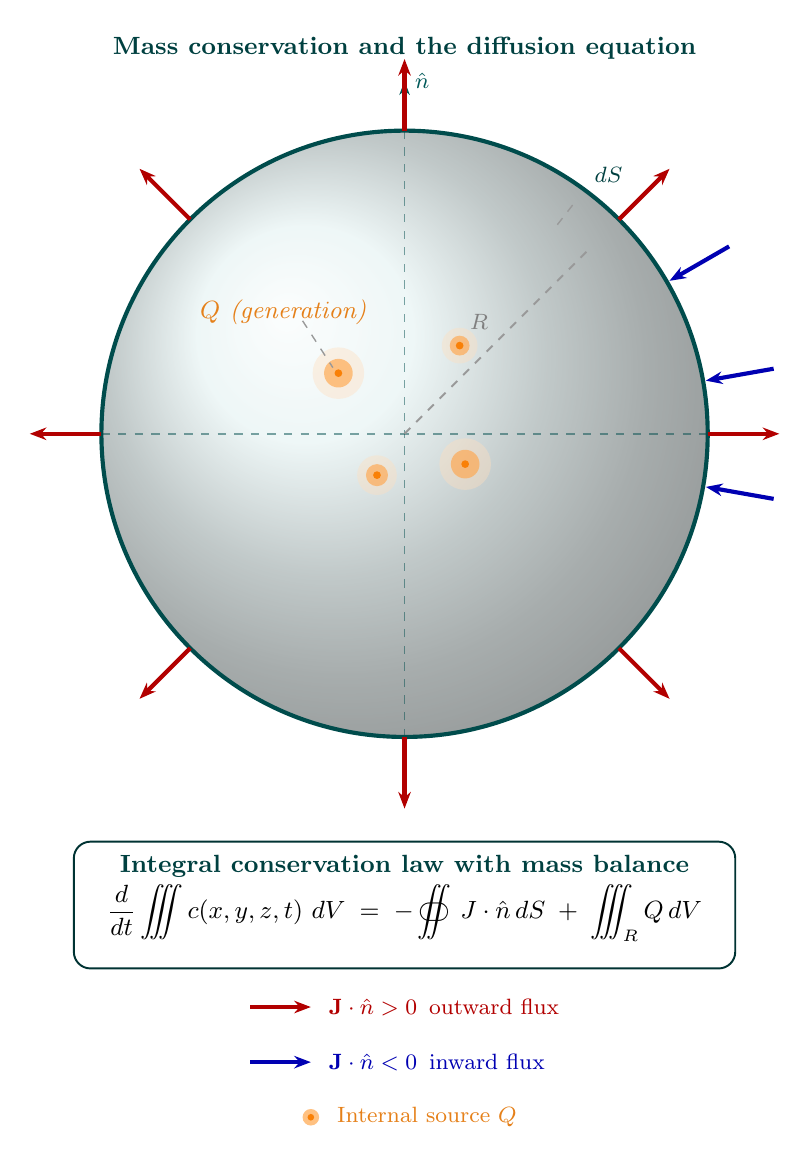
\begin{tikzpicture}[
	  scale=0.7,
	  every node/.style={font=\small},
	  outarrow/.style={-{Stealth[length=6pt]}, line width=1.5pt, color=red!70!black},
	  inarrow/.style={-{Stealth[length=6pt]}, line width=1.5pt, color=blue!70!black},
	  leader/.style={dashed, line width=0.5pt, color=black!40},
	  axis/.style={dashed, line width=0.6pt, color=teal!60!black, opacity=0.5},
	]

	%% ── Sphere ──────────────────────────────────────────────────────────────
	\def\R{5.5cm}
	\coordinate (O) at (0,0);

	\shade[ball color=teal!15, opacity=0.6] (O) circle (\R);
	\draw[teal!60!black, line width=1.5pt] (O) circle (\R);

	\draw[axis] (-\R,0) -- (\R,0);
	\draw[axis] (0,-\R) -- (0,\R);

	%% ── Internal generation sources ────────────────────────────────────────
	\foreach \x/\y/\r in {-1.2/1.1/0.26, 1.1/-0.55/0.26, -0.5/-0.75/0.20, 1.0/1.6/0.18}{
	  \fill[orange!25, opacity=0.4] (\x,\y) circle (\r*1.8 cm);
	  \fill[orange!70, opacity=0.65] (\x,\y) circle (\r cm);
	  \fill[orange!90!brown] (\x,\y) circle (0.07 cm);
	}

	\node[font=\small\itshape, color=orange!60!brown] at (-2.2, 2.2)
	  {$Q$ (generation)};
	\draw[leader] (-1.85,2.05) -- (-1.3,1.2);

	%% ── Surface normal ──────────────────────────────────────────────────────
	\draw[-{Stealth[length=5pt]}, teal!70!black, line width=1pt]
	  (0,\R) -- (0,\R+0.9cm) node[right, font=\footnotesize\itshape]{$\hat{n}$};

	\node[font=\footnotesize, color=teal!50!black] at (3.7, 4.7) {$dS$};
	\draw[leader] (3.05,4.15) -- (2.7,3.7);

	\draw[black!40, dashed, line width=0.7pt] (O) -- (3.4,3.4)
	  node[midway, above left, font=\footnotesize\itshape, black!50]{$R$};

	%% ── Outward flux arrows ─────────────────────────────────────────────────
	\foreach \angle in {90, 45, 0, -45, -90, -135, 180, 135}{
	  \draw[outarrow]
	    ({cos(\angle)*\R},{sin(\angle)*\R})
	    -- ({cos(\angle)*(\R+1.3cm)},{sin(\angle)*(\R+1.3cm)});
	}

	%% ── Inward flux arrows ──────────────────────────────────────────────────
	\foreach \angle in {30, 10, -10}{
	  \draw[inarrow]
	    ({cos(\angle)*(\R+1.3cm)},{sin(\angle)*(\R+1.3cm)})
	    -- ({cos(\angle)*(\R+0.05cm)},{sin(\angle)*(\R+0.05cm)});
	}

	%% ── Mass balance equation ────────────────────────────────────────────────
	\draw[teal!40!black, rounded corners=6pt, line width=0.7pt]
	  (-6.0,-9.7) rectangle (6.0,-7.4);

	\node[font=\small\bfseries, teal!50!black] at (0,-7.85)
	  {Integral conservation law with mass balance};

	\node[font=\small] at (0,-8.7)
	  {$\displaystyle\frac{d }{dt}\iiint c\!\left( x,y,z,t \right) \, dV
	    \;=\; -\oiint\,\pmb{J}\cdot\hat{n}\, dS
	    \;+\; \iiint_{R} Q \, dV$};

	%% ── Legend (below equation box) ─────────────────────────────────────────
	\begin{scope}[yshift=-10.4cm]
	  % Outward
	  \draw[outarrow] (-2.8, 0) -- (-1.7, 0);
	  \node[right, font=\footnotesize, color=red!70!black] at (-1.55, 0)
	    {$\mathbf{J}\cdot\hat{n}>0$\enspace outward flux};

	  % Inward
	  \draw[inarrow] (-2.8, -1) -- (-1.7, -1);
	  \node[right, font=\footnotesize, color=blue!70!black] at (-1.55, -1)
	    {$\mathbf{J}\cdot\hat{n}<0$\enspace inward flux};

	  % Generation dot
	  \fill[orange!70, opacity=0.7]  (-1.7, -2) circle (0.15cm);
	  \fill[orange!90!brown]         (-1.7, -2) circle (0.06cm);
	  \node[right, font=\footnotesize, color=orange!60!brown] at (-1.4, -2)
	    {Internal source $Q$};
	\end{scope}

	%% ── Title ────────────────────────────────────────────────────────────────
	\node[font=\small\bfseries, teal!50!black] at (0, 7.0)
	  {Mass conservation and the diffusion equation};

	\end{tikzpicture}
	\end{center}
	Mathematically, we triply integrate over the concentration to derive the total amount of pollutant in the volume, and differentiate to get the rate of change.
	\[
		\text{rate of change of amount of pollutant} = \frac{d }{dt}\iiint_{R} c \!\left( x,y,z,t \right) \, dV
	\]
	This is balanced by the sum of the net flux of the pollutant across the volume boundary and the total amount internally generated, which is given by
	\[
		-\oiint\, \pmb{J}\cdot \hat{n} \, dS + \iiint_{R} Q \, dV 
	\]
	where \( \hat{n} \) is the unit vector normal to the surface of the volume and \( Q \) is the amount of pollutant internally generated per unit volume per unit time. By the divergence theorem, the surface integral can be rewritten as 
	\[
		=\iiint_{R} \nabla \cdot \pmb{J} \, dV 
	\]
	Combining the terms, we have
	\[
		\frac{d }{dt}\iiint_{R} c \!\left( x,y,z,t \right) \, dV = -\iiint_{R} \nabla \cdot \pmb{J} \, dV + \iiint_{R} Q \, dV
	\]
	Assembling the integrands together on one side yields
	\[
		\frac{\partial c}{\partial t} + \nabla \cdot \pmb{J} - Q = 0 
	\]
	And using Fick's law in three dimensions as derived in part (b)
	\[
		\pmb{J} = -k \nabla c
	\]
	We derive the diffusion equation
	\[
		\frac{\partial c}{\partial t} - k\nabla^{2}c - Q = 0
	\]
\end{enumerate}

% QUESTION 2
\qs{1.5.2}{For conduction of thermal energy, the heat flux vector is \( \pmb{\phi} = -K_{0}\nabla u \). If in addition the molecules move at an average velocity \( \pmb{V} \), a process called \textbf{convection}, then briefly explain why \( \pmb{\phi} = -K_{0}\nabla u + c \rho u \pmb{V} \). Derive the corresponding equation for heat flow, including both conduction and convection of thermal energy (assuming constant thermal properties with no sources).}

Fundamentally, this is a superposition argument. \textbf{The total flux is the sum of the energy transfer anti-parallel to the temperature gradient (conduction) and the ``movement'' of energy by the physical translation of the molecules (convection).}

\begin{center}
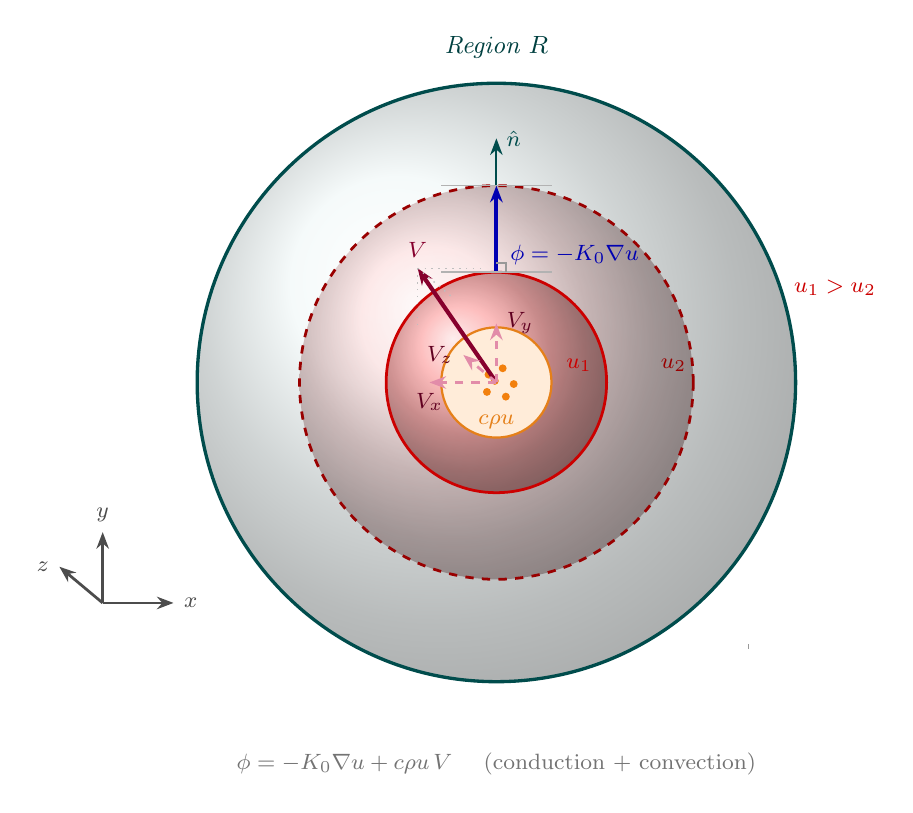
\begin{tikzpicture}[
  every node/.style={font=\small},
  arr/.style={-{Stealth[length=6pt]}, line width=1.5pt},
  leader/.style={dashed, line width=0.5pt, color=black!40},
  axis/.style={dashed, line width=0.6pt, color=black!30},
]

\def\Ra{3.8cm}
\def\RaI{2.5cm}
\def\RaII{1.4cm}

\coordinate (O) at (0,0);

%% ── Concentric spheres ───────────────────────────────────────────────────
\shade[ball color=teal!10, opacity=0.5] (O) circle (\Ra);
\draw[teal!60!black, line width=1.2pt] (O) circle (\Ra);

\shade[ball color=red!20, opacity=0.55] (O) circle (\RaI);
\draw[red!60!black, line width=1pt, dashed] (O) circle (\RaI);

\shade[ball color=red!50, opacity=0.6] (O) circle (\RaII);
\draw[red!80!black, line width=1pt] (O) circle (\RaII);

%% ── Level surface labels ─────────────────────────────────────────────────
\node[font=\footnotesize, red!80!black] at (1.05, 0.22) {$u_1$};
\node[font=\footnotesize, red!60!black] at (2.25, 0.22) {$u_2$};

%% ── Conduction flux arrow: radially outward at top, clearly normal ───────
%% Arrow goes straight up from u1 surface to u2 surface — visibly orthogonal
%% to the (locally horizontal) level curves
\draw[arr, color=blue!70!black]
  (0, 1.4) -- (0, 2.5)
  node[right, font=\footnotesize, color=blue!70!black, xshift=1pt, yshift=-25pt]
  {$\pmb{\phi} = -K_0 \nabla u$};

%% Small normal tick label
\draw[arr, teal!60!black, line width=0.8pt]
  (0, 2.5) -- (0, 3.1)
  node[right, font=\footnotesize\itshape, teal!60!black]{$\hat{n}$};

%% Tangent line to level surface u1 at top — makes orthogonality explicit
\draw[black!30, line width=0.6pt] (-0.7, 1.4) -- (0.7, 1.4);
%% Tangent line to level surface u2 at top
\draw[black!30, line width=0.6pt] (-0.7, 2.5) -- (0.7, 2.5);
%% Right-angle mark at base of arrow
\draw[black!40, line width=0.6pt] (0.12, 1.4) -- (0.12, 1.52) -- (0, 1.52);

%% ── 3D coordinate axes — bottom-left corner, well clear of everything ────
\coordinate (Axes) at (-5.0, -2.8);
\def\axlen{0.9}

\draw[arr, black!70, line width=1pt]
  (Axes) -- ++(\axlen, 0) node[right, font=\footnotesize]{$x$};
\draw[arr, black!70, line width=1pt]
  (Axes) -- ++(0, \axlen) node[above, font=\footnotesize]{$y$};
\draw[arr, black!70, line width=1pt]
  (Axes) -- ++(-0.55, 0.46) node[left, font=\footnotesize]{$z$};

%% ── Molecule sub-sphere — bottom-right, outside main sphere ─────────────
\coordinate (Msph) at (0, 0);
\def\Rm{0.7cm}

\draw[fill=orange!15, draw=orange!60!brown, line width=0.8pt]
  (Msph) circle (\Rm);

%% Molecule dots
\foreach \mx/\my in {-0.1/0.1, 0.08/0.18, 0.22/-0.02,
                      -0.12/-0.12, 0.12/-0.18, -0.02/0.02}{
  \fill[orange!80!brown] (\mx, \my) circle (0.05cm);
}

%% c rho u label — below the sub-sphere so it doesn't crowd the vectors
\node[font=\footnotesize, orange!60!brown] at (0, -0.5)
  {$c\rho u$};
\draw[leader] (3.2, -3.38) -- (3.2, -3.32);

%% ── Velocity vector V and projections ───────────────────────────────────
%% V points upper-left from sub-sphere
\coordinate (Vtip) at (-1.0, 1.45);
\draw[arr, color=purple!70!black, line width=1.5pt]
  (Msph) -- (Vtip)
  node[above, font=\footnotesize, color=purple!70!black]{$\pmb{V}$};

%% Vx: horizontal left
\draw[arr, purple!45, line width=1pt, dashed]
  (Msph) -- ++(-0.85, 0)
  node[below, font=\footnotesize, color=purple!50!black]{$V_x$};

%% Vy: vertical up
\draw[arr, purple!45, line width=1pt, dashed]
  (Msph) -- ++(0, 0.75)
  node[right, font=\footnotesize, color=purple!50!black]{$V_y$};

%% Vz: oblique (isometric z direction)
\draw[arr, purple!45, line width=1pt, dashed]
  (Msph) -- ++(-0.42, 0.35)
  node[left, font=\footnotesize, color=purple!50!black]{$V_z$};

%% Construction lines from tip to foot of each projection
\draw[dotted, black!25, line width=0.5pt] (Vtip) -- ++(0.85, 0);
\draw[dotted, black!25, line width=0.5pt] (Vtip) -- ++(0, -0.75);
\draw[dotted, black!25, line width=0.5pt] (Vtip) -- ++(0.42, -0.35);

%% ── Labels ───────────────────────────────────────────────────────────────
\node[font=\small\itshape, teal!50!black] at (0, 4.25) {Region $R$};

\node[font=\footnotesize, red!80!black] at (4.3, 1.2)
  {$u_1 > u_2$};

\node[font=\footnotesize, black!55] at (0, -4.85)
   {$\pmb{\phi} = -K_0\nabla u + c\rho u\,\pmb{V}$
   \quad (conduction + convection)};

\end{tikzpicture}
\end{center}

The addition of the \( c \rho u \pmb{V} \) term arises from the notion of ``advecting'' energy across space in each of the three spatial dimensions, \textit{in addition} to the spontaneous energy transfer (i.e. heat) in the direction of the negative temperature gradient. We can confirm that \( c \rho u \pmb{V} \) is also in units of flux:
\[
	\!\left( \frac{\text{J}}{\text{m}^{3}} \right) \!\left( \frac{\text{m}}{\text{s}} \right) = \frac{\text{J}}{\text{m}^{2} \cdot \text{s}}
\]
Hence total flux is 
\[
	\pmb{\phi} = -K_{0}\nabla u + c \rho u \pmb{V} 
\]
Substituting into the derivation of the heat equation (with no sources) produces
\begin{align*}
	c \rho \frac{\partial u}{\partial t} & = -\nabla \cdot \!\left( -K_{0}\nabla u + c \rho u \pmb{V} \right) \\
	 & = K_{0}\nabla^{2}u - c \rho \!\left( \pmb{V} \cdot \nabla u + u \!\left( \nabla \cdot \pmb{V} \right) \right)
\end{align*}
But by premise, \( \pmb{V} \) is constant, so that last term vanishes. Dividing through by \( c \rho \) and using \( k = K_{0} / c \rho \), we derive
\[
	\frac{\partial u}{\partial t} = k \nabla^{2}u - \pmb{V} \cdot \nabla u
\]
We typically call the first term \textbf{diffusion} and the second \textbf{advection}.

\vspace{12pt}

% QUESTION 3
\qs{1.5.3}{Consider the polar coordinates
\begin{align*}
	x & = r \cos\!\left(\theta\right) \\
	y & = r \sin\!\left(\theta\right)
\end{align*}
\begin{enumerate}[label=(\alph*)]
	\item Since \( r^{2} = x^{2} + y^{2} \), show that \( \frac{\partial r}{\partial x} = \cos\!\left(\theta\right) \), \( \frac{\partial r}{\partial y} = \sin\!\left(\theta\right) \), \( \frac{\partial \theta}{\partial y} = \frac{\cos\!\left(\theta\right)}{r} \), and \( \frac{\partial \theta}{\partial x} = \frac{-\sin\!\left(\theta\right)}{r} \).
	\item Show that \( \pmb{\hat{r}} = \cos\!\left(\theta\right) \pmb{\hat{i}} + \sin\!\left(\theta\right) \pmb{\hat{j}} \) and \( \pmb{\hat{\theta}} = -\sin\!\left(\theta\right)\pmb{\hat{i}} + \cos\!\left(\theta\right)\pmb{\hat{j}} \).
	\item Using the chain rule, show that \( \nabla = \pmb{\hat{r}}\frac{\partial }{\partial r} + \pmb{\hat{\theta}}\frac{1}{r}\frac{\partial }{\partial \theta} \) and hence \( \nabla u = \frac{\partial u}{\partial r}\pmb{\hat{r}} + \frac{1}{r}\frac{\partial u}{\partial \theta}\pmb{\hat{\theta}} \).
	\item If \( \pmb{A} = A_{r}\pmb{\hat{r}} + A_{\theta}\pmb{\hat{\theta}} \), show that \( \nabla \cdot \pmb{A} = \frac{1}{r}\frac{\partial }{\partial r}\!\left( r A_{r} \right) + \frac{1}{r}\frac{\partial }{\partial \theta}\!\left( A_{\theta} \right) \), since \( \partial \pmb{\hat{r}} / \partial \theta = \pmb{\hat{\theta}} \) and \( \partial \pmb{\hat{\theta}} / \partial \theta = -\pmb{\hat{r}} \) follows from part (b).
	\item Show that \( \nabla^{2}u = \frac{1}{r}\frac{\partial }{\partial r}\!\left( r \frac{\partial u}{\partial r} \right) + \frac{1}{r^{2}}\frac{\partial^{2}u}{\partial \theta^{2}} \).
\end{enumerate}}

\begin{enumerate}[label=(\alph*)]
	\item \begin{alignat}{3}
		&& 2r \frac{\partial r}{\partial x} & = 2x \frac{\partial x}{\partial x} = 2r \cos\!\left(\theta\right) && \implies \frac{\partial r}{\partial x} = \cos\!\left(\theta\right) \\
		&& 2r \frac{\partial r}{\partial y} & = 2y \frac{\partial y}{\partial y} = 2r \sin\!\left(\theta\right) && \implies \frac{\partial r}{\partial y} = \sin\!\left(\theta\right) \\
		&& \frac{\partial y}{\partial y} & = \frac{\partial r}{\partial y}\sin\!\left(\theta\right) + r \cos\!\left(\theta\right) \frac{\partial \theta}{\partial y} && \notag \\
		&&			      & = \sin^{2}\!\left(\theta\right) + r \cos\!\left(\theta\right) \frac{\partial \theta}{\partial y} \notag \\
		&& 1 & = 1 - \cos^{2}\!\left(\theta\right) + r \cos\!\left(\theta\right) \frac{\partial \theta}{\partial y} \notag \\
		\implies && \cos^{2}\!\left(\theta\right) & = r \cos\!\left(\theta\right) \frac{\partial \theta}{\partial y} && \implies \frac{\partial \theta}{\partial y} = \frac{\cos\!\left(\theta\right)}{r} \\
			 && \frac{\partial x}{\partial x} & = \frac{\partial r}{\partial x}\cos\!\left(\theta\right) - r \sin\!\left(\theta\right) \frac{\partial \theta}{\partial x} && \notag \\
			 && 				  & = \cos^{2}\!\left(\theta\right) - r \sin\!\left(\theta\right) && \notag \\
			 && 1 & = 1 - \sin^{2}\!\left(\theta\right) - r \sin\!\left(\theta\right) \frac{\partial \theta}{\partial x} \notag  \\
		\implies && \sin^{2}\!\left(\theta\right) & = -r \sin\!\left(\theta\right) \frac{\partial \theta}{\partial x} && \implies \frac{\partial \theta}{\partial x} = -\frac{\sin\!\left(\theta\right)}{r}
	\end{alignat}
	\item Let \( \pmb{r} = r \cos\!\left(\theta\right) \pmb{\hat{i}} + r \sin\!\left(\theta\right) \pmb{\hat{j}} \). By the Pythagorean theorem, its norm is
	\[
		\abs{\pmb{r}} = \sqrt{r^{2}\cos^{2}\!\left(\theta\right) + r^{2}\sin^{2}\!\left(\theta\right) } = r
	\]
	Normalizing, we derive
	\[
		\pmb{\hat{r}} = \frac{\pmb{r}}{\abs{\pmb{r}}} = \cos\!\left(\theta\right) \pmb{\hat{i}} + \sin\!\left(\theta\right) \pmb{\hat{j}} 
	\]
	Now, we know that \( \pmb{\hat{r}} \) and \( \pmb{\hat{\theta}} \) must be spanning basis vectors, which is to say that we must have \( \pmb{\hat{r}} \perp \pmb{\hat{\theta}} \). We need only differentiate with respect to \( \theta \) to derive this orthogonal basis vector.
	\[
		\pmb{\hat{\theta}} = -\sin\!\left(\theta\right) \pmb{\hat{i}} + \cos\!\left(\theta\right) \pmb{\hat{j}} 
	\]
	\item In \( x \) and \( y \) coordinates, by definition
	\[
		\nabla = \frac{\partial }{\partial x}\pmb{\hat{i}} + \frac{\partial }{\partial y}\pmb{\hat{j}} 
	\]
	Let \( u \!\left( r,\theta \right) \) be a function of \( r \) and \( \theta \). Consider the total derivatives with respect to \( x \) and \( y \):
	\begin{align*}
		\frac{\partial u}{\partial x} & = \frac{\partial u}{\partial r}\frac{\partial r}{\partial x} + \frac{\partial u}{\partial \theta}\frac{\partial \theta}{\partial x} \\
		 			      & = \frac{\partial u}{\partial r}\cos\!\left(\theta\right) - \frac{\partial u}{\partial \theta}\frac{1}{r}\sin\!\left(\theta\right) \\ 
		 			      & = \!\left( \cos\!\left(\theta\right) \frac{\partial }{\partial r} - \frac{1}{r}\sin\!\left(\theta\right)\frac{\partial }{\partial \theta} \right)u \\
		\frac{\partial u}{\partial y} & = \frac{\partial u}{\partial r}\frac{\partial r}{\partial y} + \frac{\partial u}{\partial \theta}\frac{\partial \theta}{\partial y} \\
					      & = \frac{\partial u}{\partial r}\sin\!\left(\theta\right) + \frac{\partial u}{\partial \theta}\frac{1}{r}\cos\!\left(\theta\right) \\
					      & = \!\left( \sin\!\left(\theta\right) \frac{\partial }{\partial r} + \frac{1}{r}\cos\!\left(\theta\right) \frac{\partial }{\partial \theta} \right)u
	\end{align*}
	Combining these expressions for \( \partial u / \partial x \) and \( \partial u / \partial y \), we have the anticipated result
	\begin{align*}
		\nabla u & = \frac{\partial u}{\partial r} \!\left[ \cos\!\left(\theta\right) \pmb{\hat{i}} + \sin\!\left(\theta\right) \pmb{\hat{j}} \right] + \frac{1}{r}\frac{\partial u}{\partial \theta} \!\left[ -\sin\!\left(\theta\right) \pmb{\hat{i}} + \cos\!\left(\theta\right) \pmb{\hat{j}} \right] \\
			 & = \frac{\partial u}{\partial r}\pmb{\hat{r}} + \frac{1}{r}\frac{\partial u}{\partial \theta}\pmb{\hat{\theta}}
	\end{align*}
	\item The key physical intuition is that the purpose of polar coordinates is to represent \textit{radial symmetry}, and particularly, a frame of reference that \textit{rotates} while retaining the orthogonality of the basis vectors. Put differently, the axes move with rotation, unlike in the Cartesian case, where the positions of \( \pmb{\hat{i}} \) and \( \pmb{\hat{j}} \) are fixed.

	Instead of component-wise multiplication as we can afford to do in the Cartesian case, we must completely expand the dot product and calculate term-by-term.
	\begin{align*}
		\nabla \cdot A & = \!\left( \pmb{\hat{r}}\frac{\partial }{\partial r} + \pmb{\hat{\theta}}\frac{1}{r}\frac{\partial }{\partial \theta} \right) \cdot \!\left( A_{r}\pmb{\hat{r}} + A_{\theta}\pmb{\hat{\theta}} \right) \\
		 & = \pmb{\hat{r}}\frac{\partial }{\partial r}\!\left( A_{r}\pmb{\hat{r}} \right) + \pmb{\hat{r}}\frac{\partial }{\partial r}\!\left( A_{\theta}\pmb{\hat{\theta}} \right) + \pmb{\hat{\theta}}\frac{1}{r}\frac{\partial }{\partial \theta}\!\left( A_{r}\pmb{\hat{r}} \right) + \pmb{\hat{\theta}}\frac{1}{r}\frac{\partial }{\partial \theta}\!\left( A_{\theta}\pmb{\hat{\theta}} \right) \\ 
		 & = \pmb{\hat{r}}\!\left( \frac{\partial A_{r}}{\partial r}\pmb{\hat{r}} + A_{r}\frac{\partial \pmb{\hat{r}}}{\partial r} \right) + \pmb{\hat{r}}\!\left( \frac{\partial A_{\theta}}{\partial r}\pmb{\hat{\theta}} + A_{\theta}\frac{\partial \pmb{\hat{\theta}}}{\partial r} \right) + \pmb{\hat{\theta}}\frac{1}{r}\!\left( \frac{\partial A_{r}}{\partial \theta}\pmb{\hat{r}} + A_{r}\frac{\partial \pmb{\hat{r}}}{\partial \theta} \right) \\
		 & \qquad + \pmb{\hat{\theta}}\frac{1}{r}\!\left( \frac{\partial A_{\theta}}{\partial \theta}\pmb{\hat{\theta}} + A_{\theta}\frac{\partial \pmb{\hat{\theta}}}{\partial \theta} \right) \\
		 & = \frac{\partial A_{r}}{\partial r} + \frac{A_{r}}{r} + \frac{1}{r}\frac{\partial A_{\theta}}{\partial \theta} \\
		 & = \frac{1}{r}\!\left( \frac{\partial }{\partial r}\!\left( rA_{r} \right) + \frac{\partial A_{\theta}}{\partial \theta} \right)
	\end{align*}
	where we use the facts that \( \partial \pmb{\hat{r}} / \partial \theta = \pmb{\hat{\theta}} \), \( \partial \pmb{\hat{\theta}} / \partial \theta = -\pmb{\hat{r}} \), and \( \pm \pmb{\hat{r}} \cdot \pm \pmb{\hat{\theta}} = 0 \).
	\item Calculate the Laplacian as 
	\begin{align*}
		\nabla^{2} = \nabla \cdot \nabla & = \!\left( \pmb{\hat{r}}\frac{\partial }{\partial r} + \pmb{\hat{\theta}}\frac{1}{r}\frac{\partial }{\partial \theta} \right) \cdot \!\left( \pmb{\hat{r}}\frac{\partial }{\partial r} + \pmb{\hat{\theta}}\frac{1}{r}\frac{\partial }{\partial \theta} \right) \\
		 & = \pmb{\hat{r}}\frac{\partial }{\partial r}\!\left( \pmb{\hat{r}}\frac{\partial }{\partial r} \right) + \pmb{\hat{r}}\frac{\partial }{\partial r}\!\left( \pmb{\hat{\theta}}\frac{1}{r}\frac{\partial }{\partial \theta} \right) + \pmb{\hat{\theta}}\frac{1}{r}\frac{\partial }{\partial \theta}\!\left( \pmb{\hat{r}}\frac{\partial }{\partial r} \right) \\ 
		 & \qquad + \pmb{\hat{\theta}}\frac{1}{r}\frac{\partial }{\partial \theta}\!\left( \pmb{\hat{\theta}}\frac{1}{r}\frac{\partial }{\partial \theta} \right) \\ 
		 & = \pmb{\hat{r}}\!\left( \frac{\partial \pmb{\hat{r}}}{\partial r}\frac{\partial }{\partial r} + \pmb{\hat{r}}\frac{\partial^2 }{\partial r^2} \right) + \pmb{\hat{\theta}}\frac{1}{r}\!\left( \frac{\partial \pmb{\hat{r}}}{\partial \theta}\frac{\partial }{\partial r} + \pmb{\hat{r}}\frac{\partial }{\partial \theta}\frac{\partial }{\partial r} \right) \\
		 & \qquad + \pmb{\hat{\theta}}\frac{1}{r^2}\!\left( \frac{\partial \pmb{\hat{\theta}}}{\partial \theta}\frac{\partial }{\partial \theta} + \pmb{\hat{\theta}}\frac{\partial^2 }{\partial \theta^2} \right) \\
		 & = \frac{\partial^2 }{\partial r^2} + \frac{1}{r}\frac{\partial }{\partial r} + \frac{1}{r^{2}}\frac{\partial^2 }{\partial \theta^2} \\
		 & = \frac{1}{r}\frac{\partial }{\partial r}\!\left( r \frac{\partial }{\partial r} \right) + \frac{1}{r^{2}}\frac{\partial^2 }{\partial \theta^2}
	\end{align*}
	where in cases where the operator is \( \partial / \partial r \), the unit vector is pulled out, and if multiplied by its orthogonal unit vector, the entire term vanishes. Then \( \nabla^{2}u = \frac{1}{r}\frac{\partial }{\partial r}\!\left( r \frac{\partial u}{\partial r} \right) + \frac{1}{r^{2}}\frac{\partial^2 u}{\partial \theta^2} \).
\end{enumerate}

% QUESTION 4
\qs{1.5.4}{Using Exercise 1.5.3(a) and the chain rule for partial derivatives, derive the special case of Exercise 1.5.3(e) if \( u \!\left( r \right) \) only.}

Begin with
\[
	\nabla^{2}u = \frac{\partial^2 u}{\partial x^2} + \frac{\partial^2 u}{\partial y^2}
\]
To calculate the second derivatives of \( u \), refer to 1.5.3(c) and apply the chain rule once more. Since here \( u \!\left( r \right) \) is not a function of \( \theta \), we omit the terms involving it.
\begin{align*}
	\frac{\partial^2 u}{\partial x^2} & = \frac{\partial }{\partial x}\!\left( \frac{\partial u}{\partial r}\frac{\partial r}{\partial x} + \frac{\partial u}{\partial \theta}\frac{\partial \theta}{\partial x} \right) \\
	 & = \frac{\partial^2 u}{\partial r^2}\!\left( \frac{\partial r}{\partial x} \right)^{2} + \frac{\partial u}{\partial r}\frac{\partial^2 r}{\partial x^2} \\
	\frac{\partial^2 u}{\partial y^2} & = \frac{\partial }{\partial y}\!\left( \frac{\partial u}{\partial r}\frac{\partial r}{\partial y} + \frac{\partial u}{\partial \theta}\frac{\partial \theta}{\partial y} \right) \\
	 & = \frac{\partial^2 u}{\partial r^2}\!\left( \frac{\partial r}{\partial y} \right)^{2} + \frac{\partial u}{\partial r}\frac{\partial^2 r}{\partial y^2}
\end{align*}
To get the second derivatives of \( r \), refer to 1.5.3(a) and differentiate once more:
\begin{alignat*}{3}
	\frac{\partial }{\partial x}\!\left( 2r \frac{\partial r}{\partial x} \right) & = \frac{\partial }{\partial x}\!\left( 2x \right) && && \\
	\implies 2 \!\left( \frac{\partial r}{\partial x} \right)^{2} + 2r \frac{\partial^2 r}{\partial x^2} & = 2 && \implies \frac{\partial^2 r}{\partial x^2} && = \frac{1 - \!\left( \partial r / \partial x \right)^{2}}{r} = \frac{1 - \cos^{2}\!\left(\theta\right)}{r} \\
													     & && && = \boxed{\frac{\sin^{2}\!\left(\theta\right)}{r}} \\ 
	\frac{\partial }{\partial y}\!\left( 2r \frac{\partial r}{\partial y} \right) & = \frac{\partial }{\partial y}\!\left( 2y \right) && && \\
	\implies 2 \!\left( \frac{\partial r}{\partial y} \right)^{2} + 2r \frac{\partial^2 r}{\partial y^2} & = 2 && \implies \frac{\partial^2 r}{\partial y^2} && = \frac{1 - \!\left( \partial r / \partial y \right)^{2}}{r} = \frac{1 - \sin^{2}\!\left(\theta\right)}{r} \\ 
													     & && && = \boxed{\frac{\cos^{2}\!\left(\theta\right)}{r}}
\end{alignat*}
Now adding the second derivatives of \( u \), derive
\begin{align*}
	\nabla^{2}u & = \frac{\partial^2 u}{\partial x^2} + \frac{\partial^2 u}{\partial y^2} \\
		    & = \frac{\partial^2 u}{\partial r^2}\!\left[ \!\left( \frac{\partial r}{\partial x} \right)^{2} + \!\left( \frac{\partial r}{\partial y} \right)^{2} \right] + \frac{\partial u}{\partial r}\!\left[ \frac{\partial^2 r}{\partial x^2} + \frac{\partial^2 r}{\partial y^2} \right] \\ 
		    & = \frac{\partial^2 u}{\partial r^2}\!\left[ \cos^{2}\!\left(\theta\right) + \sin^{2}\!\left(\theta\right) \right] + \frac{1}{r}\frac{\partial u}{\partial r}\!\left[ \sin^{2}\!\left(\theta\right) + \cos^{2}\!\left(\theta\right) \right] \\
		    & = \frac{\partial^2 u}{\partial r^2} + \frac{1}{r}\frac{\partial u}{\partial r}
\end{align*}
Now, the easiest solution would have been to substitute into the result of 1.5.3(e), in which case we have
\[
	\nabla^{2}u = \frac{\partial^2 u}{\partial r^2} + \frac{1}{r}\frac{\partial u}{\partial r} 
\]
Since there is no variation with \( \theta \), the final \( 1 / r^{2} \frac{\partial^2 u}{\partial \theta^2} \) term vanishes.

\vspace{12pt}

% QUESTION 5
\qs{1.5.5}{Assume that the temperature is circularly symmetric: \( u = u \!\left( r,t \right) \), where \( r^{2} = x^{2} + y^{2} \). We will derive the heat equation for this problem. Consider any circular annulus \( a \le r \le b \).
\begin{enumerate}[label=(\alph*)]
	\item Show that the total heat energy is \( 2 \pi \int^{b}_{a} c \rho u r \, dr \).
	\item Show that the flow of heat energy per unit time out of the annulus at \( r = b \) is \( -2 \pi b K_{0} \partial u / \partial r \big|_{r = b} \). A similar result holds at \( r = a \).
	\item Use parts (a) and (b) to derive the circularly symmetric heat equation without sources:
	\[
		\frac{\partial u}{\partial t} = \frac{k}{r}\frac{\partial }{\partial r}\!\left( r \frac{\partial u}{\partial r} \right) 
	\]
\end{enumerate}}

\begin{enumerate}[label=(\alph*)]
	\item The first observation to make here is since the annulus is a two-dimensional creature, the energy density \( c \rho u \) is in units of energy per area. The infinitesimal area is \( r\,dr\,d \theta \), apparent from the diagram below:
	\begin{center}
	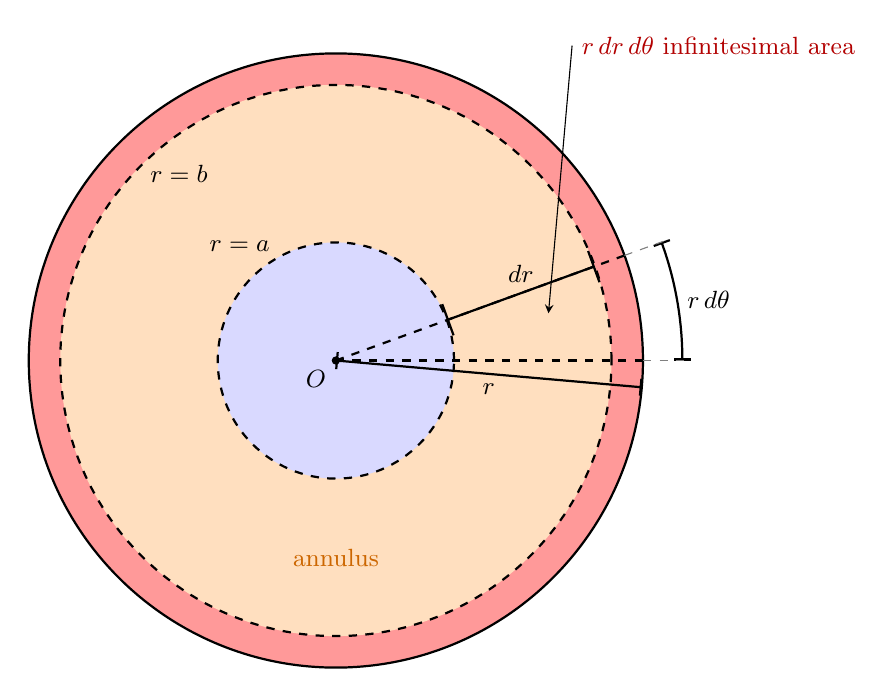
\begin{tikzpicture}[>=stealth]
	    % Full disk (r < a) — blue
	    \fill[blue!15] (0,0) circle (1.5cm);
	    % Annulus (a < r < b) — orange
	    \fill[orange!25] (0,0) circle (3.5cm);
	    \fill[blue!15] (0,0) circle (1.5cm);
	    % Thin strip (r to r+dr) — red, between 3.5 and 3.9
	    \fill[red!40] (0,0) circle (3.9cm);
	    \fill[orange!25] (0,0) circle (3.5cm);
	    \fill[blue!15] (0,0) circle (1.5cm);
	    % Borders
	    \draw[thick, dashed] (0,0) circle (1.5cm);
	    \draw[thick, dashed] (0,0) circle (3.5cm);
	    \draw[thick] (0,0) circle (3.9cm);
	    % Labels r=a and r=b
	    \node[font=\small] at (130:1.9cm) {$r=a$};
	    \node[font=\small] at (130:3.1cm) {$r=b$};
	    % Radial lines for the strip wedge
	    \draw[dashed, thick] (0,0) -- (0:3.9cm);
	    \draw[dashed, thick] (0,0) -- (20:3.9cm);
	    % Label r: slightly below horizontal, from origin to r=b
	    \draw[|-|, thick] (0,0) -- (-5:3.9cm)
		node[midway, below, font=\small] {$r$};
	    % Label dr: continues from r=b to dashed circle
	    \draw[{Bar[width=12pt]}-{Bar[width=12pt]}, thick] (20:1.5cm) -- (20:3.5cm)
		node[midway, above, font=\small] {$dr$};
	    % Label r*dtheta along arc, outside at radius 4.4cm
	    \draw[|-|, thick] (0:4.4cm) arc[start angle=0, end angle=20, radius=4.4cm]
		node[midway, right, font=\small] {$r\,d\theta$};
	    % Leader lines
	    \draw[dashed, gray] (0:3.9cm) -- (0:4.5cm);
	    \draw[dashed, gray] (20:3.9cm) -- (20:4.5cm);
	    % Strip label
	    \draw[->] (3.0, 4.0) node[right, font=\small, red!70!black] {$r\,dr\,d \theta$ infinitesimal area}
		-- (2.7, 0.6);
	    % Annulus label
	    \node[font=\small, orange!80!black] at (0.0, -2.5) {annulus};
	    % Origin
	    \fill (0,0) circle (1.5pt) node[below left, font=\small] {$O$};
	\end{tikzpicture}
	\end{center}
	The arc length, \( r\,d \theta \) gives the width of the infinitesimal area, while \( dr \) gives its length. Since we consider the whole rotational span of the annulus going from \( 0 \) to \( 2 \pi \), the total energy is given by
	\[
		\text{total heat energy} = \int^{2 \pi}_{0} \int^{b}_{a} c \rho u r \, dr \, d \theta = 2 \pi \int^{b}_{a} c \rho u r \, dr 
	\]
	\item The intuition here is to recall that in the case of the rod, heat flux is in units of thermal energy per unit time per unit \textit{surface area}; for this two-dimensional annulus, its circumference, a one-dimensional quantity, means flux is now in terms of unit \textit{length}. To represent flow of heat energy per unit time, we need to multiply Fourier's heat law by a length: the circumference, or \( 2 \pi b \).
	\[
		\vcenter{\hbox{\shortstack{flow of heat energy \\ per unit time}}}
		= 
		-2 \pi b K_{0} \frac{\partial u}{\partial r} \Big|_{r=b}
	\]
	Similarly, we can calculate for \( r = a \)
	\[
		\vcenter{\hbox{\shortstack{flow of heat energy \\ per unit time}}}
		= 
		-2 \pi a K_{0} \frac{\partial u}{\partial r} \Big|_{r=a} 
	\]
	Heat flows \textit{out} at \( r = b \) and \textit{in} at \( r = a \).

	In general, the rate of flow of heat energy is given by
	\[
		\phi r \Delta \theta = -K_{0}r \frac{\partial u}{\partial r} \Delta \theta 
	\]
	where \( r \Delta \theta \) is the arc length over which flux transpires.
	\item Assuming no sources, derive the circular heat equation with the integral conservation setup 
	\begin{align*}
		\frac{d }{dt}\int^{2 \pi}_{0} \int^{b}_{a} c \rho u r \, dr \, d \theta & = \phi \!\left( a,t \right)L_{a} - \phi \!\left( b,t \right)L_{b} \\
											& = -2 \pi a K_{0}\frac{\partial u}{\partial r}\Big|_{a} + 2 \pi b K_{0}\frac{\partial u}{\partial r}\Big|_{b}
	\end{align*}
	Conceptually, the rate of change of total energy equals the difference in inbound and outbound energy transfer through the annulus. On the right side, we can equivalently write (thanks to the Fundamental Theorem of Calculus)
	\[
		\frac{d }{dt}\int^{2 \pi}_{0} \int^{b}_{a} c \rho u r \, dr \, d \theta = K_{0}\int^{2 \pi}_{0} \int^{b}_{a} \frac{\partial }{\partial r} \!\left( r \frac{\partial u}{\partial r} \right) \, dr \, d \theta 
	\]
	Moving the differential operator on the left into the integrand (since we do not integrate over time) and setting the integrands equal, we have
	\[
		c \rho \frac{\partial u}{\partial t}r = K_{0}\frac{\partial }{\partial r}\!\left( r \frac{\partial u}{\partial r} \right) 
	\]
	Divide through by \( c \rho r \) to conclude
	\[
		\frac{\partial u}{\partial t} = \frac{k}{r}\frac{\partial }{\partial r}\!\left( r \frac{\partial u}{\partial r} \right) 
	\]
\end{enumerate}

\newpage
% QUESTION 6
\qs{1.5.6}{Modify Exercise 1.5.5 if the thermal properties depend on \( r \).}

The integral conservation law becomes
\begin{align*}
	\frac{d }{d t}\int^{2 \pi}_{0} \int^{b}_{a} c \!\left( r \right)\rho \!\left( r \right)u \!\left( r,t \right) r \, dr \, d \theta & = \phi \!\left( a,t \right)L_{a} - \phi \!\left( b,t \right)L_{b} \\
	 & = -2 \pi a K_{0}\!\left( a \right)\frac{\partial u}{\partial r}\Big|_{a} + 2 \pi b K_{0}\!\left( b \right)\frac{\partial u}{\partial r}\Big|_{b}
\end{align*}
which then becomes
\[
	\frac{d }{d t}\int^{2 \pi}_{0} \int^{b}_{a} c \!\left( r \right)\rho \!\left( r \right)u \!\left( r,t \right) r \, dr \, d \theta = \int^{2 \pi}_{0} \int^{b}_{a} \frac{\partial }{\partial r}\!\left( K_{0}\!\left( r \right)r \frac{\partial u}{\partial r} \right) \, dr \, d \theta  
\]
Notice here that \( K_{0}\!\left( r \right) \), now a function of \( r \), can no longer be pulled out of the integrand. Moving the derivative inside the integral on the left and setting the integrands equal yields
\[
	c \!\left( r \right) \rho \!\left( r \right) \frac{\partial u}{\partial r} \!\left( r,t \right) r = \frac{\partial }{\partial r}\!\left( K_{0}\!\left( r \right)r \frac{\partial u}{\partial r} \right) 
\]
Lastly, divide by \( c \!\left( r \right) \rho \!\left( r \right) r \) to get
\[
	\frac{\partial u}{\partial t} = \frac{1}{c \!\left( r \right) \rho \!\left( r \right) r} \frac{\partial }{\partial r}\!\left( K_{0}\!\left( r \right) r \frac{\partial u}{\partial r} \right) 
\]

% QUESTION 7
\qs{1.5.7}{Derive the heat equation in two dimensions by using Green's theorem, (1.5.16), the two-dimensional form of the divergence theorem.}

In general, for any two-dimensional geometric object \( R \), the rate of change of the total energy is given by
\[
	\frac{d }{dt}\iint_{R} c \rho u \, dS
\]
where \( \rho \) is an area density and \( dS \) is an infinitesimal area. Let \( \pmb{\hat{\phi}} \) be the heat flux per time per length. The total flux through the line boundary is
\[
	-\oint \pmb{\phi} \cdot \pmb{\hat{n}} \, d \tau
\]
Assuming a non-zero source, assembling the integral conservation law gives us
\[
	\frac{d }{dt}\iint_{R} c \rho u \, dS = -\oint \pmb{\phi} \cdot \pmb{\hat{n}} \, d \tau + \iint_{R} Q \, dS
\]
It is easiest to convert the line integral to the divergence theorem in two dimensions by way of Green's theorem:
\[
	\iint_{R} \nabla \cdot \pmb{\phi} \, dS = \oint \pmb{\phi} \cdot \pmb{\hat{n}} \, d \tau
\]
which allows us to write and consolidate the integrands to derive
\begin{align*}
	\frac{d }{dt}\iint_{R} c \rho u \, dS & = -\iint_{R} \nabla \cdot \pmb{\phi} \, dS + \iint_{R} Q \, dS \\
	c \rho \frac{\partial u}{\partial t} & = -\nabla \cdot \pmb{\phi} + Q
\end{align*}
and finally, substituting Fourier's heat law \( \pmb{\phi} = -K_{0} \nabla u \) and dividing by \( c \rho \) produces the heat equation
\[
	\frac{\partial u}{\partial t} = k \nabla^{2}u + \frac{Q}{c \rho}
\]

% QUESTION 8
\qs{1.5.8}{If Laplace's equation is satisfied in three dimensions, show that
\[
	\oiint \nabla u \cdot \pmb{\hat{n}} \, dS = 0 
\]
for any closed surface. (\textit{Hint}: Use the divergence theorem.) Give a physical interpretation of this result (in the context of heat flow).}

By premise, \( \nabla^{2}u = 0 \). Using the divergence theorem, we can write
\[
	\oiint \nabla u \cdot \pmb{\hat{n}} \, dS = \iiint_{R} \nabla \cdot \nabla u \, dV = \iiint_{R} \nabla^{2}u \, dV = 0
\]
Physically, if \( \pmb{\phi} \propto \nabla u \), then this says that the net flux is zero. If there are no internal sources, then the \textit{rate of change of total energy is zero.}

\vspace{12pt}

% QUESTION 9
\qs{1.5.9}{Determine the equilibrium temperature distribution inside a circular annulus (\( r_{1} \le r \le r_{2} \)):
\begin{enumerate}[label=(\alph*)]
	\item if the outer radius is at temperature \( T_{2} \) and the inner at \( T_{1} \)
	\item if the outer radius is insulated and the inner radius is at temperature \( T_{1} \)
\end{enumerate}}

\begin{enumerate}[label=(\alph*)]
	\item By premise, \( u \!\left( r_{1},t \right) = T_{1} \) and \( u \!\left( r_{2},t \right) = T_{2} \). At equilibrium, we assume
	\[
		\frac{\partial u}{\partial t} = 0 
	\]
	Then we solve
	\[
		\frac{\partial }{\partial r}\!\left( r \frac{\partial u}{\partial r} \right) = \frac{\partial u}{\partial r} + r \frac{\partial^2 u}{\partial r^2} = 0
	\]
	Effectively, this is a homogeneous second-order ordinary differential equation, which we can rewrite as 
	\[
		\frac{d^2 u}{d r^2} + \frac{1}{r}\frac{d u}{d r} = 0 
	\]
	An Euler-Cauchy equation, we know to substitute \( u = r^{n} \) to find
	\[
		n \!\left( n - 1 \right) r^{n-2} + n r^{n-2} = 0 \quad \implies \quad n^{2} = 0
	\]
	Which leaves a repeated root in \( n = 0 \). Thus one null solution is \( u_{1} = 1 \). A second-order equation implies two linearly independent solutions. To find the other, we use reduction of order. Let \( u_{2} = v \!\left( r \right) u_{1} = v \!\left( r \right) \). Then 
	\[
		v'' + \frac{1}{r}v' = 0 
	\]
	Now, let \( w = v' \). Then we rewrite as 
	\[
		w' + \frac{1}{r}w = 0 
	\]
	Separating variables, solve
	\[
		\int \frac{dw}{w} = -\int \frac{dr}{r} \quad \implies \quad \ln\!\left(w\right) = -\ln\!\left(r\right) \quad \implies \quad w = \frac{1}{r}
	\]
	which implies \( u_{2} = v \!\left( r \right) = \ln\!\left(r\right) \). Our complete null solution is
	\[
		u \!\left( r \right) = c_{1} + c_{2}\ln\!\left(r\right)  
	\]
	Using this solution, we can write the system of equations
	\begin{align*}
		u \!\left( r_{1} \right) & = c_{1} + c_{2}\ln\!\left(r_{1}\right) = T_{1} \\
		u \!\left( r_{2} \right) & = c_{1} + c_{2}\ln\!\left(r_{2}\right) = T_{2}
	\end{align*}
	Solving for the unknowns gives
	\[
		c_{1} = \frac{T_{1}\ln\!\left(r_{2}\right) - T_{2}\ln\!\left(r_{1}\right)}{\ln\!\left(r_{2}/r_{1}\right)}, \quad c_{2} = \frac{T_{2} - T_{1}}{\ln\!\left(r_{2}/r_{1}\right) }
	\]
	\item By premise, \( \partial u / \partial r |_{r=r_{2}} = 0 \) and \( u \!\left( r_{1},t \right) = T_{1} \). From the general solution obtained in the previous part 
	\[
		u \!\left( r \right) = c_{1} + c_{2}\ln\!\left(r\right)  
	\]
	we generate the system of equations
	\begin{align*}
		u \!\left( r_{1} \right) & = c_{1} + c_{2}\ln\!\left(r_{1}\right) = T_{1} \\
		\frac{\partial u}{\partial r}\Big|_{r=r_{2}} & = \frac{c_{2}}{r_{2}} = 0 
	\end{align*}
	which implies \( c_{1} = T_{1} \) and \( c_{2} = 0 \). Then \( u \!\left( r \right) = T_{1} \). Interestingly, since heat cannot transfer out of the annulus at \( r = r_{2} \), the temperature must equilibriate to a constant value throughout the entire region.
\end{enumerate}

% QUESTION 10
\qs{1.5.10}{Determine the equilibrium temperature distribution inside a circle (\( r \le r_{0} \)) if the boundary is fixed at temperature \( T_{0} \).}

By premise, \( u \!\left( r_{0} \right) = T_{0} \). We can derive the general solution as we did before
\[
	u \!\left( r \right) = c_{1} + c_{2}\ln\!\left(r\right)  
\]
But a problem arises when we consider the origin of the circle at \( r = 0 \) -- the temperature approaches infinity, a physical impossibility. Therefore, we require a second ``boundary condition'' of sorts, namely
\[
	\abs{u \!\left( r \right)} < \infty \text{ for all } r 
\]
Since we cannot satisfy this boundary condition with the logarithm's presence, we necessarily force \( c_{2} = 0 \). That leaves
\[
	u \!\left( r_{0} \right) = c_{1} = T_{0} \quad \implies \quad u \!\left( r \right) = T_{0}
\]
Intuitively, this makes physical sense. For a constant fixed temperature at the boundary, we must have homogeneous temperature throughout the circle at equilibrium.

\vspace{12pt}

% QUESTION 11
\qs{1.5.11}{Consider
\[
	\frac{\partial u}{\partial t} = \frac{k}{r}\frac{\partial }{\partial r}\!\left( r \frac{\partial u}{\partial r} \right), \quad a < r < b 
\]
subject to
\[
	u \!\left( r,0 \right) = f \!\left( r \right), \frac{\partial u}{\partial r}\!\left( a,t \right) = \beta, \text{ and } \frac{\partial u}{\partial r}\!\left( b,t \right) = 1
\]
Using physical reasoning, for what value(s) of \( \beta \) does an equilibrium temperature distribution exist?}

The temperature at equilibrium is given by the general form
\[
	u \!\left( r \right) = c_{1} + c_{2}\ln\!\left(r\right)  
\]
which subjected to the boundary conditions yields
\begin{align*}
	\frac{\partial u}{\partial r}\!\left( a,t \right) & = \frac{c_{2}}{a} = \beta \\
	\frac{\partial u}{\partial r}\!\left( b,t \right) & = \frac{c_{2}}{b} = 1
\end{align*}
This immediately implies \( c_{2} = b \) and \( \beta = b / a \). Previously, we derived that the heat flow is proportional to
\[
	r \frac{\partial u}{\partial r} 
\]
In our case, we can see that form at \( r = a \):
\[
	\frac{\partial u}{\partial r}\!\left( a,t \right) = \beta = \frac{b}{a} \quad \implies \quad a \frac{\partial u}{\partial r}\!\left( a,t \right) = b 
\]

% QUESTION 12
\qs{1.5.12}{Assume that the temperature is spherically symmetric, \( u = u \!\left( r,t \right) \), where \( r \) is the distance from a fixed point (\( r^{2} = x^{2} + y^{2} + z^{2} \)). Consider the heat flow (without sources) between any two concentric spheres of radii \( a \) and \( b \).
\begin{enumerate}[label=(\alph*)]
	\item Show that the total heat energy is \( 4 \pi \int^{b}_{a} c \rho u r^{2} \, dr \).
	\item Show that the flow of heat energy per unit time out of the spherical shell at \( r = b \) is \( -4 \pi b^{2}K_{0} \partial u / \partial r |_{r = b} \). A similar result holds at \( r = a \).
	\item Use parts (a) and (b) to derive the spherically symmetric heat equation
	\[
		\frac{\partial u}{\partial t} = \frac{k}{r^{2}}\frac{\partial }{\partial r}\!\left( r^{2}\frac{\partial u}{\partial r} \right) 
	\]
\end{enumerate}}

The diagram below visualizes heat flow through the concentric spheres:

\begin{center}
\begin{tikzpicture}[>=stealth]

    % Shell (a <= r <= b) — orange
    \shade[ball color=orange!30, opacity=0.8] (0,0) circle (3.5cm);

    % Inner sphere (r < a) — blue
    \shade[ball color=blue!40, opacity=1.0] (0,0) circle (2.0cm);

    % Equator ellipses for 3D feel
    \draw[black!40, dashed] (0,0) ellipse (3.5cm and 0.6cm);
    \draw[black!30, dashed] (0,0) ellipse (2.0cm and 0.35cm);

    % Longitude arc on outer sphere
    \draw[black!20] (0, 3.5) arc[start angle=90, end angle=270, radius=3.5cm];
    \draw[black!20, dashed] (0, 3.5) arc[start angle=90, end angle=-90, radius=3.5cm];

    % Borders — only two
    \draw[thick] (0,0) circle (3.5cm);         % r = b
    \draw[thick, dashed] (0,0) circle (2.0cm); % r = a

    % Labels
    \node[font=\small] at (135:2.5cm) {$r=a$};
    \node[font=\small] at (135:4.0cm) {$r=b$};

    % Radial line
    \draw[thick] (0,0) -- (0:3.5cm);

    % Outward normal
    \draw[->, thick] (0:3.5cm) -- (0:4.2cm)
        node[right, font=\small] {$\hat{n}$};

    % Heat flux arrow
    \draw[->, thick, blue!70!black] (0:2.0cm) -- (0:2.7cm)
        node[above, font=\small, blue!70!black] {$-K_0\dfrac{\partial u}{\partial r}$};

    % Shell label
    \draw[->] (3.2, -2.8) node[right, font=\small, orange!80!black] {shell $a < r < b$}
        -- (2.6, -0.5);

    % Origin
    \fill (0,0) circle (1.5pt) node[below left, font=\small] {$O$};

    % 3D axes
    \coordinate (Ax) at (-4.5, -3.2);
    \draw[->, black!70, thick] (Ax) -- ++(1.0, 0)    node[right, font=\footnotesize]{$x$};
    \draw[->, black!70, thick] (Ax) -- ++(0, 1.0)    node[above, font=\footnotesize]{$y$};
    \draw[->, black!70, thick] (Ax) -- ++(-0.6, 0.5) node[left,  font=\footnotesize]{$z$};

\end{tikzpicture}
\end{center}

\begin{enumerate}[label=(\alph*)]
	\item Let \( x \), \( y, \), and \( z \) be defined as in (1.5.21):
	\begin{align*}
		x & = r \sin\!\left(\phi\right)\cos\!\left(\theta\right) \\
		y & = r \sin\!\left(\phi\right)\sin\!\left(\theta\right) \\ 
		z & = r \cos\!\left(\phi\right)
	\end{align*}
	One potential source of confusion is \( \phi \) is the author's nomenclature for flux \textit{and} the polar angle, but I hope the distinction is clear in the proceeding derivation. Since \( c \rho u \) is an energy density, we do a volume integral to get the total heat energy. In spherical coordinates, our set up is
	\[	
		\text{total heat energy} = \int^{2 \pi}_{0} \int^{\pi}_{0} \int^{b}_{a} c \rho u r^{2}\sin\!\left(\phi\right) \, dr \, d \phi \, d \theta  
	\]
	Integrating over \( \phi \) and \( \theta \), we derive
	\[
		4 \pi \int^{b}_{a} c \rho u r^{2} \, dr  
	\]
	Notice how the surface area of a sphere, \( 4 \pi r^{2} \), emerges in our formula.
	\item Analogous to the two-dimensional case of the annulus, since flux is given in units of energy per unit time per unit area, we multiply by the entire area through which heat transfer occurs. Since the area of the spherical shell at \( r = b \) is \( 4 \pi b^{2} \), we multiply the Fourier heat conduction law by this area.
	\[
		-4 \pi b^{2}K_{0}\frac{\partial u}{\partial r}\Big|_{r=b} 
	\]
	and similarly, the same calculation holds at \( r = a \):
	\[
		-4 \pi a^{2}K_{0}\frac{\partial u}{\partial r}\Big|_{r=a} 
	\]
	\item The integral conservation law is given by
	\begin{align*}
		\frac{d }{dt}\int^{2 \pi}_{0} \int^{\pi}_{0} \int^{b}_{a} c \rho u r^{2}\sin\!\left(\phi\right) \, dr \, d \phi \, d \theta & = \phi \!\left( a,t \right) S_{a} - \phi \!\left( b,t \right) S_{b} \\
															       & = -4 \pi a^{2}K_{0}\frac{\partial u}{\partial r}\Big|_{r=a} + 4 \pi b^{2}K_{0}\frac{\partial u}{\partial r}\Big|_{r=b} \\
															       & = \int^{2 \pi}_{0} \int^{\pi}_{0} \int^{b}_{a} \frac{\partial }{\partial r}\!\left( K_{0}r^{2}\sin\!\left(\phi\right)\frac{\partial u}{\partial r} \right) \, dr \, d \phi \, d \theta 
	\end{align*}
	Setting the integrands equal produces
	\[
		c \rho \frac{\partial u}{\partial t}r^{2}\sin\!\left(\phi\right) = \frac{\partial }{\partial r}\!\left( K_{0}r^{2}\sin\!\left(\phi\right) \frac{\partial u}{\partial r} \right)
	\]
	On the right-hand side, pull out the \( K_{0} \) and \( \sin\!\left(\phi\right) \) from the derivative, as they are independent of \( r \). Divide by \( c \rho r^{2} \sin\!\left(\phi\right) \) to conclude
	\[
		\frac{\partial u}{\partial t} = \frac{k}{r^{2}}\frac{\partial }{\partial r}\!\left( r^{2}\frac{\partial u}{\partial r} \right) 
	\]
\end{enumerate}	

% QUESTION 13
\qs{1.5.13}{Determine the \textit{steady-state} temperature distribution between two concentric \textit{spheres} with radii \( 1 \) and \( 4 \), respectively, if the temperature of the outer sphere is maintained at \( 80^{\circ} \) and the inner sphere at \( 0^{\circ} \) (see Exercise 1.5.12).}

Using our result from the previous exercise, set \( \partial u / \partial t = 0 \) to derive
\[
	r^{2}\frac{\partial^2 u}{\partial r^2} + 2r \frac{\partial u}{\partial r} = 0 \quad \iff \quad \frac{\partial^2 u}{\partial r^2} + \frac{2}{r}\frac{\partial u}{\partial r} = 0
\]
Which equivalently is an second-order ordinary Euler-Cauchy homogeneous differential equation:
\[
	\frac{d^2 u}{d r^2} + \frac{2}{r}\frac{d u}{d r} = 0 
\]
Let \( u = r^{n} \). Then
\[
	n \!\left( n - 1 \right)r^{n - 2} + 2n r^{n - 2} = 0 \quad \implies \quad n^{2} + n = 0 \quad \implies \quad n_{1} = 0, n_{2} = -1
\]
which produces the general solution
\[
	u \!\left( r \right) = c_{1} + c_{2}\frac{1}{r}
\]
Imposing the boundary conditions, we have the system of equations
\begin{align*}
	u \!\left( 1 \right) & = c_{1} + c_{2} = 0 \\
	u \!\left( 4 \right) & = c_{1} + c_{2}\frac{1}{4} = 80
\end{align*}
In matrix form,
\[
	\begin{bmatrix}
		1 & 1\\
		1 & 1 / 4 \\
	\end{bmatrix}
	\begin{bmatrix}
		c_{1} \\
		c_{2} \\
	\end{bmatrix}
	=
	\begin{bmatrix}
		0 \\
		80 \\
	\end{bmatrix}
\]
Solving for the unknowns, we get
\[
	c_{1} = \frac{320}{3}, \quad c_{2} = -\frac{320}{3} 
\]
and equilibrium temperature distribution
\[
	u \!\left( r \right) = \frac{320}{3}\!\left( 1 - \frac{1}{r} \right) 
\]

% QUESTION 14
\qs{1.5.14}{Isobars are lines of constant temperature. Show that isobars are perpendicular to any part of the boundary that is insulated.}

I believe the author means \textbf{isotherms}, which are level curves for temperature. Isobars are for pressure. By definition, the temperature distribution along an isotherm is constant, meaning \( u \!\left( r \right) = c \). Additionally, from the construction of a gradient, we know that it is always perpendicular to level curves at any point. Along the normal vector \( \pmb{\hat{n}} \), if we have an insulated boundary, then \( \nabla u \cdot \pmb{\hat{n}} = 0 \). Since the gradient is orthogonal to both the isotherm and the normal vector, they must be parallel, demonstrating that isotherms must be orthogonal to any part of an insulated boundary.

\newpage

% QUESTION 15
\qs{1.5.15}{Derive the heat equation in three dimensions assuming constant thermal properties and no sources.}

Let \( c \) be the specific heat, \( \rho \) the mass density, and \( u \!\left( x,y,z,t \right) \) the temperature distribution. The rate of change of the total energy in the region \( R \) is
\[
	\frac{d }{dt} \iiint_{R} c \rho u \, dV 
\]
Let \( \pmb{\phi} \) be the heat flux (energy per unit time per unit area). One conceptual simplification is to measure the heat flux along the vector normal to the surface boundary, which we calculate as 
\[
	\pmb{\phi} \cdot \pmb{\hat{n}} 
\]
which has sign convention \( \pmb{\phi} \cdot \pmb{\hat{n}} < 0 \) corresponding to inward flux and \( \pmb{\phi} \cdot \pmb{\hat{n}} > 0 \) for outward flux. Summing over the aggregate of these infinitesimal areas, we have the surface integral
\[
	-\oiint \pmb{\phi} \cdot \pmb{\hat{n}} \, dS 
\]
Setting this equal to the rate of change of the total energy, we have
\[
	\frac{d }{d t}\iiint_{R} c \rho u \, dV = -\oiint \pmb{\phi} \cdot \pmb{\hat{n}} \, dS
\]
Moving the derivative inside the triple integral (as we don't integrate over time) and invoking the divergence theorem to deal with the surface integral, we have
\[
	\iiint_{R} c \rho \frac{\partial u}{\partial t} \, dV = -\iiint_{R} \nabla \cdot \pmb{\phi} \, dV
\]
At last, we can set the integrands together to derive
\[
	c \rho \frac{\partial u}{\partial t} = -\nabla \cdot \pmb{\phi} 
\]
In this final step, use the Fourier heat conduction law
\[
	\pmb{\phi} = -K_{0}\nabla u 
\]
where \( K_{0} \) is the thermal conductivity, substitute for \( \pmb{\phi} \), and divide by \( c \rho \) to get the heat equation in three dimensions
\[
	 \frac{\partial u}{\partial t} = k \nabla^{2}u
\]
where \( k = K_{0} / c \rho \) is the thermal diffusivity.

\newpage

% QUESTION 16
\qs{1.5.16}{Express the integral conservation law for any three-dimensional object. Assume there are no sources. Also assume the heat flow is specified, \( \nabla u \cdot \pmb{\hat{n}} = \pmb{g \!\left( x,y,z \right)} \), on the entire boundary and does not depend on time. By integrating with respect to time, determine the total thermal energy. (Hint: Use the initial condition.)}

As derived in the previous exercise, the integral conservation law with no sources is
\[
	\iiint_{R} c \rho \frac{\partial u}{\partial t} \, dV = -\oiint \pmb{\phi} \cdot \pmb{\hat{n}} \, dS 
\]
On the right-hand side, substituting \( \pmb{\phi} = -K_{0}\nabla u \) gives
\[
	-\oiint \pmb{\phi} \cdot \pmb{\hat{n}} \, dS = -K_{0}\oiint \nabla u \cdot \pmb{\hat{n}} \, dS = -K_{0} \oiint g \!\left( x,y,z \right) \, dS
\]
Integrating all over time, we have
\begin{align*}
	\int^{t}_{0} \!\left[ \iiint_{R} c \rho \frac{\partial u}{\partial T} \, dV \right] \, dT & = -K_{0}\int^{t}_{0} \!\left[ \oiint g \!\left( x,y,z \right) \, dS \right] \, dT \\
	\implies \iiint_{R} c \rho u \!\left( x,y,z,t \right) \, dV & = \iiint_{R} c \rho f \!\left( x,y,z \right) \, dV - K_{0}\!\left[ \oiint g \!\left( x,y,z \right) \, dS \right]t 
\end{align*}
where we use the fact that from the initial condition,
\[
	\iiint_{R} c \rho u \!\left( x,y,z,0 \right) \, dV = \iiint_{R} c \rho f \!\left( x,y,z \right) \, dV 
\]

% QUESTION 17
\qs{1.5.17}{Derive the integral conservation law for any three dimensional object (with constant thermal properties) by integrating the heat equation (1.5.11) (assuming no sources). Show that the result is equivalent to (1.5.1).}

Integrate over volume on both sides of the heat equation to derive
\[
	\iiint_{R} c \rho \frac{\partial u}{\partial t} \, dV = K_{0}\iiint_{R} \nabla \cdot \nabla u \, dV 
\]
where \( k = K_{0} / c \rho \) was split into its constituent terms and \( c \rho \) multiplied on both sides. On the right, use the Fourier heat conduction law and substitute:
\[
	\iiint_{R} c \rho \frac{\partial u}{\partial t} \, dV = -\iiint_{R} \nabla \cdot \pmb{\phi} \, dV 
\]
Lastly, use the divergence theorem to restore equation (1.5.1).
\[
	\iiint_{R} c \rho \frac{\partial u}{\partial t} \, dV = -\oiint \pmb{\phi} \cdot \pmb{\hat{n}} \, dS 
\]

\textbf{Orthogonal curvilinear coordinates}. A coordinate system \( \!\left( u,v,w \right) \) may be introduced and defined by \( x = x \!\left( u,v,w \right) \), \( y = y \!\left( u,v,w \right) \), and \( z = z \!\left( u,v,w \right) \). The radial vector \( \pmb{r} \equiv x \pmb{\hat{i}} + y \pmb{\hat{j}} + z \pmb{\hat{k}} \). Partial derivatives of \( \pmb{r} \) with respect to a coordinate are in the direction of the coordinate. Thus, for example, a vector in the \( u \)-direction \( \partial \pmb{r} / \partial u \) can be made a unit vector \( \pmb{\hat{e}_{u}} \) in the \( u \)-direction by dividing by its length \( h_{u} = \abs{\partial \pmb{r} / \partial u} \) called the \textbf{scale factor}: \( \pmb{\hat{e}_{u}} = \frac{1}{h_{u}}\partial \pmb{r} / \partial u \).

\vspace{12pt}

% QUESTION 18
\qs{1.5.18}{Determine the scale factors for the cylindrical coordinates.}

Define the radial vector \( \pmb{r} \) as above. The coordinate transformation is as given in equation (1.5.18). The scale factors and transformed unit vectors are as follows:
\begin{align*}
	\frac{\partial \pmb{r}}{\partial r} & = \frac{\partial x}{\partial r}\pmb{\hat{i}} + \frac{\partial y}{\partial r}\pmb{\hat{j}} + \frac{\partial z}{\partial r}\pmb{\hat{k}} \\
	 & = \cos\!\left(\theta\right) \pmb{\hat{i}} + \sin\!\left(\theta\right) \pmb{\hat{j}} \\ 
	h_{r} & = \abs{\partial \pmb{r} / \partial r} = \sqrt{\cos^{2}\!\left(\theta\right) + \sin^{2}\!\left(\theta\right)} = \boxed{1} \\
	\pmb{\hat{e}_{r}} & = \frac{1}{h_{r}}\frac{\partial \pmb{r}}{\partial r} = \boxed{\frac{\partial \pmb{r}}{\partial r}} \\
	\frac{\partial \pmb{r}}{\partial \theta} & = \frac{\partial x}{\partial \theta}\pmb{\hat{i}} + \frac{\partial y}{\partial \theta}\pmb{\hat{j}} + \frac{\partial z}{\partial \theta}\pmb{\hat{k}} \\
						 & = r \!\left[ -\sin\!\left(\theta\right) \pmb{\hat{i}} + \cos\!\left(\theta\right) \pmb{\hat{j}} \right] \\
	h_{\theta} & = \abs{\partial \pmb{r} / \partial \theta} = \sqrt{r^{2}\!\left[ \cos^{2}\!\left(\theta\right) + \sin^{2}\!\left(\theta\right) \right]} = \boxed{r} \\
	\pmb{\hat{e}_{\theta}} & = \frac{1}{h_{\theta}}\frac{\partial \pmb{r}}{\partial \theta} = \boxed{\frac{1}{r}\frac{\partial \pmb{r}}{\partial \theta}} \\
	\frac{\partial \pmb{r}}{\partial z} & = \frac{\partial z}{\partial z}\pmb{\hat{k}} = \pmb{\hat{k}} \\
	h_{z} & = \abs{\partial \pmb{r} / \partial z} = \boxed{1} \\
	\pmb{\hat{e}_{z}} & = \frac{1}{h_{z}}\frac{\partial \pmb{r}}{\partial z} = \boxed{\pmb{\hat{k}}}
\end{align*}

% QUESTION 19
\qs{1.5.19}{Determine the scale factors for spherical coordinates.}

Define the radial vector \( \pmb{r} \) as above. The coordinate transformation is as given in equation (1.5.21). The scale factors and transformed unit vectors are as follows:
\begin{align*}
	\frac{\partial \pmb{r}}{\partial \rho} & = \frac{\partial x}{\partial \rho}\pmb{\hat{i}} + \frac{\partial y}{\partial \rho}\pmb{\hat{j}} + \frac{\partial z}{\partial \rho}\pmb{\hat{k}} \\
	 & = \sin\!\left(\phi\right)\cos\!\left(\theta\right)\pmb{\hat{i}} + \sin\!\left(\phi\right)\sin\!\left(\theta\right)\pmb{\hat{j}} + \cos\!\left(\phi\right)\pmb{\hat{k}} \\ 
	h_{\rho} & = \abs{\partial \pmb{r} / \partial \rho} = \sqrt{\sin^{2}\!\left(\phi\right)\cos^{2}\!\left(\theta\right) + \sin^{2}\!\left(\phi\right)\sin^{2}\!\left(\theta\right) + \cos^{2}\!\left(\phi\right)} = \boxed{1} \\
	\pmb{\hat{e}_{\rho}} & = \frac{1}{h_{\rho}}\frac{\partial \pmb{r}}{\partial \rho} = \boxed{\frac{\partial \pmb{r}}{\partial \rho}} \\
	\frac{\partial \pmb{r}}{\partial \phi} & = \frac{\partial x}{\partial \phi}\pmb{\hat{i}} + \frac{\partial y}{\partial \phi}\pmb{\hat{j}} + \frac{\partial z}{\partial \phi}\pmb{\hat{k}} \\
					       & = \rho \cos\!\left(\phi\right) \cos\!\left(\theta\right) \pmb{\hat{i}} + \rho \cos\!\left(\phi\right) \sin\!\left(\theta\right) \pmb{\hat{j}} - \rho \sin\!\left(\phi\right) \pmb{\hat{k}} \\
	h_{\phi} & = \abs{\partial \pmb{r} / \partial \phi} = \rho \sqrt{\cos^{2}\!\left(\phi\right) \cos^{2}\!\left(\theta\right) + \cos^{2}\!\left(\phi\right) \sin^{2}\!\left(\theta\right) + \sin^{2}\!\left(\phi\right) } = \boxed{\rho} \\
	\pmb{\hat{e}_{\phi}} & = \frac{1}{h_{\phi}}\frac{\partial \pmb{r}}{\partial \phi} = \boxed{\frac{1}{\rho}\frac{\partial \pmb{r}}{\partial \phi}} \\
	\frac{\partial \pmb{r}}{\partial \theta} & = \frac{\partial x}{\partial \theta}\pmb{\hat{i}} + \frac{\partial y}{\partial \theta}\pmb{\hat{j}} + \frac{\partial z}{\partial \theta}\pmb{\hat{k}} \\
						 & = -\rho \sin\!\left(\phi\right) \sin\!\left(\theta\right) \pmb{\hat{i}} + \rho \sin\!\left(\phi\right) \cos\!\left(\theta\right) \pmb{\hat{j}} \\
	h_{\theta} & = \abs{\partial \pmb{r} / \partial \theta} = \rho \sqrt{\sin^{2}\!\left(\phi\right) \sin^{2}\!\left(\theta\right) + \sin^{2}\!\left(\phi\right) \cos^{2}\!\left(\theta\right) } = \boxed{\rho \sin\!\left(\phi\right)} \\
	\pmb{\hat{e}_{\theta}} & = \frac{1}{h_{\theta}}\frac{\partial \pmb{r}}{\partial \theta} = \boxed{\frac{1}{\rho \sin\!\left(\phi\right)}\frac{\partial \pmb{r}}{\partial \theta}}
\end{align*}

% QUESTION 20
\qs{1.5.20}{The gradient of a scalar can be expressed in terms of the new coordinate system \( \nabla g = a \partial \pmb{r} / \partial u + b \partial \pmb{r} / \partial v + c \partial \pmb{r} / \partial w \), where you will determine the scalars \( a \), \( b \), \( c \). Using \( dg = \nabla g \cdot d \pmb{r} \), derive that the \textbf{gradient} in an orthogonal curvilinear coordinate system is given by
\begin{equation}
	\nabla g = \frac{1}{h_{u}}\frac{\partial g}{\partial u}\pmb{\hat{e}_{u}} + \frac{1}{h_{v}}\frac{\partial g}{\partial v}\pmb{\hat{e}_{v}} + \frac{1}{h_{w}}\frac{\partial g}{\partial w}\pmb{\hat{e}_{w}}
	\tag{1.5.23}
\end{equation}
An expression for the divergence is more difficult to derive, and we will just state that if a vector \( \pmb{p} \) is expressed in terms of this new coordinate system \( \pmb{p} = p_{u}\pmb{\hat{e}_{u}} + p_{v}\pmb{\hat{e}_{v}} + p_{w}\pmb{\hat{e}_{w}} \), then the \textbf{divergence} satisfies
\begin{equation}
	\nabla \cdot \pmb{p} = \frac{1}{h_{u}h_{v}h_{w}}\!\left[ \frac{\partial }{\partial u}\!\left( h_{v}h_{w}p_{u} \right) + \frac{\partial }{\partial v}\!\left( h_{u}h_{w}p_{v} \right) + \frac{\partial }{\partial w}\!\left( h_{u}h_{v}p_{w} \right) \right]
	\tag{1.5.24}
\end{equation}}

The basis vectors in \( u \), \( v \), and \( w \) coordinates are
\[
	\pmb{\hat{e}_{u}} = \frac{1}{h_{u}}\frac{\partial \pmb{r}}{\partial u}, \quad \pmb{\hat{e}_{v}} = \frac{1}{h_{v}}\frac{\partial \pmb{r}}{\partial v}, \quad \pmb{\hat{e}_{w}} = \frac{1}{h_{w}}\frac{\partial \pmb{r}}{\partial w} 
\]
And the differentials are 
\begin{align*}
	dg & = \frac{\partial g}{\partial u}du + \frac{\partial g}{\partial v}dv + \frac{\partial g}{\partial w}dw \\
	d \pmb{r} & = \frac{\partial \pmb{r}}{\partial u}du + \frac{\partial \pmb{r}}{\partial v}dv + \frac{\partial \pmb{r}}{\partial w}dw \\ 
		  & = h_{u}du \, \pmb{\hat{e}_{u}} + h_{v}dv \, \pmb{\hat{e}_{v}} + h_{w}dw \, \pmb{\hat{e}_{w}}
\end{align*}
where the last equality stems from the definition of the basis vectors. Calculating \( \nabla g \cdot d \pmb{r} \) and invoking orthogonality between the basis vectors, we find
\[
	\nabla g \cdot d \pmb{r} = h^{2}_{u}a \, du + h^{2}_{v}b \, dv + h^{2}_{w}c \, dw 
\]
Setting equal to \( dg \), we can derive
\[
	\frac{\partial g}{\partial u} = h^{2}_{u}a, \quad \frac{\partial g}{\partial v} = h^{2}_{v}b, \quad \frac{\partial g}{\partial w} = h^{2}_{w}c 
\]
Back to the definition of \( \nabla g \). If we isolate \( a \), \( b \), and \( c \) and each of the derivatives of \( \pmb{r} \) from the basis vectors, we can conclude
\[
	\nabla g = \frac{1}{h_{u}}\frac{\partial g}{\partial u}\pmb{\hat{e}_{u}} + \frac{1}{h_{v}}\frac{\partial g}{\partial v}\pmb{\hat{e}_{v}} + \frac{1}{h_{w}}\frac{\partial g}{\partial w}\pmb{\hat{e}_{w}}
\]

% QUESTION 21
\qs{1.5.21}{Using (1.5.23) and (1.5.24), derive the \textbf{Laplacian} in an orthogonal curvilinear coordinate system:
\begin{equation}
	\nabla^{2}T = \frac{1}{h_{u}h_{v}h_{w}}\!\left[ \frac{\partial }{\partial u}\!\left( \frac{h_{v}h_{w}}{h_{u}}\frac{\partial T}{\partial u} \right) + \frac{\partial }{\partial v}\!\left( \frac{h_{u}h_{w}}{h_{v}}\frac{\partial T}{\partial v} \right) + \frac{\partial }{\partial w}\!\left( \frac{h_{u}h_{v}}{h_{w}}\frac{\partial T}{\partial w} \right) \right] 
	\tag{1.5.25}
\end{equation}}

Replace the components of \( \pmb{p} \) with those of \( \nabla g \), switching out \( g \) for \( T \), from (1.5.23):
\[
	p_{u} \implies \frac{1}{h_{u}}\frac{\partial T}{\partial u}, \quad p_{v} \implies \frac{1}{h_{v}}\frac{\partial T}{\partial v}, \quad p_{w} \implies \frac{1}{h_{w}}\frac{\partial T}{\partial w} 
\]
And then substitute in equation (1.5.24):
\[
	\nabla \cdot \nabla T = \nabla^{2}T = \frac{1}{h_{u}h_{v}h_{w}}\!\left[ \frac{\partial }{\partial u}\!\left( \frac{h_{v}h_{w}}{h_{u}}\frac{\partial T}{\partial u} \right) + \frac{\partial }{\partial v}\!\left( \frac{h_{u}h_{w}}{h_{v}}\frac{\partial T}{\partial v} \right) + \frac{\partial }{\partial w}\!\left( \frac{h_{u}h_{v}}{h_{w}}\frac{\partial T}{\partial w} \right) \right] 
\]

% QUESTION 22
\qs{1.5.22}{Using (1.2.25), derive the Laplacian for cylindrical coordinates.}

Let \( u = r \), \( v = \theta \), and \( w = z \). Recall from exercise 18 that the scale factors are
\[
	h_{r} = 1, \quad h_{\theta} = r, \quad h_{z} = 1 
\]
Substituting into (1.5.25) yields
\begin{align*}
	\nabla^{2}T & = \frac{1}{h_{r}h_{\theta}h_{z}}\!\left[ \frac{\partial }{\partial r}\!\left( \frac{h_{\theta}h_{z}}{h_{r}}\frac{\partial T}{\partial r} \right) + \frac{\partial }{\partial \theta}\!\left( \frac{h_{r}h_{z}}{h_{\theta}}\frac{\partial T}{\partial \theta} \right) + \frac{\partial }{\partial z}\!\left( \frac{h_{r}h_{\theta}}{h_{z}}\frac{\partial T}{\partial z} \right) \right] \\
	 & = \frac{1}{r}\!\left[ \frac{\partial }{\partial r}\!\left( r \frac{\partial T}{\partial r} \right) + \frac{\partial }{\partial \theta}\!\left( \frac{1}{r}\frac{\partial T}{\partial \theta} \right) + \frac{\partial }{\partial z}\!\left( r \frac{\partial T}{\partial z} \right) \right] \\
	 & = \frac{1}{r}\frac{\partial }{\partial r}\!\left( r \frac{\partial T}{\partial r} \right) + \frac{1}{r^{2}}\frac{\partial^2 T}{\partial \theta^2} + \frac{\partial^2 T}{\partial z^2}
\end{align*}

% QUESTION 23
\qs{1.5.23}{Using (1.5.25), derive the Laplacian for spherical coordinates.}

Let \( u = \rho \), \( v = \phi \), and \( w = \theta \). Recall from exercise 19 that the scale factors are 
\[
	h_{\rho} = 1, \quad h_{\phi} = \rho, \quad h_{\theta} = \rho \sin\!\left(\phi\right)  
\]
Substituting into (1.5.25) yields
\begin{align*}
	\nabla^{2}T & = \frac{1}{h_{\rho}h_{\phi}h_{\theta}}\!\left[ \frac{\partial }{\partial \rho}\!\left( \frac{h_{\phi}h_{\theta}}{h_{\rho}}\frac{\partial T}{\partial \rho} \right) + \frac{\partial }{\partial \phi}\!\left( \frac{h_{\rho}h_{\theta}}{h_{\phi}}\frac{\partial T}{\partial \phi} \right) + \frac{\partial }{\partial \theta}\!\left( \frac{h_{\rho}h_{\phi}}{h_{\theta}}\frac{\partial T}{\partial \theta} \right) \right] \\
	 & = \frac{1}{\rho^{2}\sin\!\left(\phi\right)}\!\left[ \frac{\partial }{\partial \rho}\!\left( \rho^{2}\sin\!\left(\phi\right) \frac{\partial T}{\partial \rho}\right) + \frac{\partial }{\partial \phi}\!\left( \sin\!\left(\phi\right) \frac{\partial T}{\partial \phi} \right) + \frac{\partial }{\partial \theta}\!\left( \frac{1}{\sin\!\left(\phi\right)}\frac{\partial T}{\partial \theta} \right) \right] \\ 
	 & = \frac{1}{\rho^{2}}\frac{\partial }{\partial \rho}\!\left( \rho^{2}\frac{\partial T}{\partial \rho} \right) + \frac{1}{\rho^{2}\sin\!\left(\phi\right)}\frac{\partial }{\partial \phi}\!\left( \sin\!\left(\phi\right) \frac{\partial T}{\partial \phi} \right) + \frac{1}{\rho^{2}\sin^{2}\!\left(\phi\right)}\frac{\partial^2 T}{\partial \theta^2}
\end{align*}

% QUESTION 24
\qs{1.5.24}{Derive the three-dimensional heat equation assuming constant thermal properties and assuming there are no sources of thermal energy. (\textit{Hint}: Use an arbitrary three-dimensional region, and use the divergence theorem.)}

The insight to make here is that the derivation of the heat equation is coordinate-agnostic. By habit we derived it in \( x \), \( y \), and \( z \) coordinates, but we could have chosen any basis. Thus refer to exercise 1.5.15.

When evaluating \( k \nabla^{2}u \), we use (1.5.25) with the appropriate scale factors.

\newpage

% QUESTION 25
\qs{1.5.25}{Suppose a sphere of radius \( 2 \) satisfies \( \frac{\partial u}{\partial t} = \nabla^{2}u + 5 \) with \( u \!\left( x,y,z,0 \right) = f \!\left( x,y,z \right) \) and on the surface of the sphere it is given that \( \nabla u \cdot \pmb{\hat{n}} = 6 \), where \( \pmb{\hat{n}} \) is a unit outward normal vector. Calculate the total thermal energy for this sphere as a function of time. (\textit{Hint}: Use the divergence theorem.)}

Using the integral conservation law and the divergence theorem, write
\begin{align*}
	\int^{t}_{0} \!\left[ \frac{d }{d t}\iiint_{R} u \!\left( x,y,z,T \right) \, dV \right] \, dT & = \!\left[ \oiint \nabla u \cdot \pmb{\hat{n}} \, dS + \iiint_{R} 5 \, dV \right]t \\
	\implies \iiint_{R} u \!\left( x,y,z,t \right) \, dV & = \iiint_{R} f \!\left( x,y,z \right) \, dV + \!\left[ \oiint 6 \, dS + \iiint_{R} 5 \, dV \right]t \\
								    & = \iiint_{R} f \!\left( x,y,z \right) \, dV + 6 \cdot 16 \pi t + 5 \cdot \frac{32}{3}\pi t \\
								    & = \iiint_{R} f \!\left( x,y,z \right) \, dV + \frac{448 \pi t}{3}
\end{align*}
Using the surface area and volume of a sphere formulae, \( S = 4 \pi r^{2} \) and \( V = \frac{4}{3}\pi r^{3} \).

\end{document}
